\documentclass[slidestop,compress,mathserif, aspectratio = 169]{beamer}
\usecolortheme{seagull} % Beamer color theme
\useinnertheme{rectangles}
\usepackage[round]{natbib}
\usepackage{bibentry}
\usepackage{graphicx}
\usepackage{epigraph}
\usepackage{makeidx}
\usepackage[]{amsmath}
\usepackage[]{amssymb}
\usepackage{color}
\usepackage{pict2e}
\usepackage{algorithm2e}
\usepackage[ngerman]{babel}
\usepackage{tikz}
\usetikzlibrary{mindmap}
\usepackage{multirow}
\usepackage[utf8]{inputenc}
\usepackage{multimedia}
\usepackage{xcolor}
\usepackage{keyval}
\usepgfmodule{shapes}
\usepackage{pgfplots}
\usepackage{sansmath}
\usepackage{pgfgantt}
\usetikzlibrary{arrows}
\usepackage{colortbl}
\usepackage{array}
\usepackage{transparent}
\usepackage{txfonts}
\usepackage{eurosym}

\graphicspath{{../../../../Vorlesungen/figures/}{./photos/}}

\makeatletter
\tikzset{
  base/.is choice,
  base/top/.code={\let\vbox\vtop},
  base/bottom/.code={\def\pgfutil@minipage[t]{\minipage[b]}},
  % base/bottom/.code={}, % for plain TeX
}
\makeatother


\definecolor{mint}{rgb}{0,172,177}

 \pgfplotsset{width=7cm, height = 7cm}

 \setbeamertemplate{section page}
{
    \begin{centering}
    \vspace{2cm}
    \begin{beamercolorbox}[sep=12pt,center]{part title}
    \usebeamerfont{title}\insertsection\par
    \end{beamercolorbox}
    \end{centering}
}



\begin{document}

\newcommand{\source}[1]{\rotatebox{90}{\tiny \color{gray} #1}}

\newcommand{\done}{${\color{teal}\checkmark}$}

%% Formalia
\title{DI Rail - Schienenfahrzeugtechnik dual studieren}
\author{Raphael Pfaff}
\institute[FH Aachen]{Fachhochschule Aachen}
\logo{\put(-18, 170){\includegraphics[width=1.4cm]{logoR}}}



{
\usebackgroundtemplate{\includegraphics[width= \paperwidth]{EmmaCastlepale}}
\frame{\titlepage}}

%\section{Fachgruppe Schienenfahrzeugtechnik}
%\frame{\vspace{1cm}
%
%\begin{center}
% \color{white} \usebeamerfont{title}{Fachgruppe Schienenfahrzeugtechnik}
%\end{center}
%}
%}
%
%\frame{\frametitle{Wer wir sind}
%\framesubtitle{Bahnerfahrung aus allen Perspektiven: Zulieferer, Hersteller, Betreiber, Wissenschaft}
%\begin{columns}[t] 
%     \begin{column}[T]{7cm} 
%     	\begin{itemize}
%     		\only<1>{\item Prof. Dr.-Ing. M. Enning:
%		\begin{itemize}
%		\item Bahnsystemtechnik
%		\item vormals RWTH Aachen
%		\item Erfahrung:
%		\begin{itemize}
%		\item Regelungstechnik
%		\item Schieneng\"uterverkehr
%		\item Kraftschlussregelungen
%		\item Zugsicherungssysteme
%		\item Netzwerke
%		\item Verkehrsz\"ahlung
%		\end{itemize}
%		\end{itemize}}
%		\only<2>{\item Prof. Dr.-Ing. B. Schmidt
%		\begin{itemize}
%		\item Bahnantriebe
%		\item vormals gro{\ss}e Unternehmensberatung
%		\item Erfahrung:
%		\begin{itemize}
%		\item Verkehrswissenschaft
%		\item Unternehmensberatung
%		\item Lebenszykluskosten
%		\item Zuverl\"assigkeit
%		\item Ausschreibungen
%		\end{itemize}
%		\end{itemize} }
%		\only<3>{\item Prof. Dr. Raphael Pfaff
%		\begin{itemize}
%		\item Schienenfahrzeugtechnik
%		\item vormals Faiveley Transport, Siemens
%		\item Erfahrung
%		\begin{itemize}
%		\item Bremssysteme
%		\item Zug- und Sto{\ss}einrichtungen
%		\item System Engineering
%		\item Konstruktionsleitung
%		\item Zuverl\"assigkeitstechnik
%		\item Claim-Management
%		\item Technischer Vertrieb
%		\end{itemize}
%		\end{itemize}}
%     	\end{itemize}
%     \end{column}
%     	\begin{column}[T]{7cm} 
%         	\begin{center}
%			\vspace{-.7cm}
%            		\includegraphics[width=0.7\textwidth]{Wir}\source{}
%        		\end{center}
%     \end{column}
% \end{columns}
%}
%
%
%
%\frame{\frametitle{CV Raphael Pfaff}
%\framesubtitle{}
%\begin{center}
%\includegraphics[height = 0.8\textheight]{CVGraphic}
%\end{center}
%}
%
%\frame{\frametitle{Wer wir sind}
%\framesubtitle{}
%\begin{center}
%\begin{tikzpicture}
%\node at (5,1) {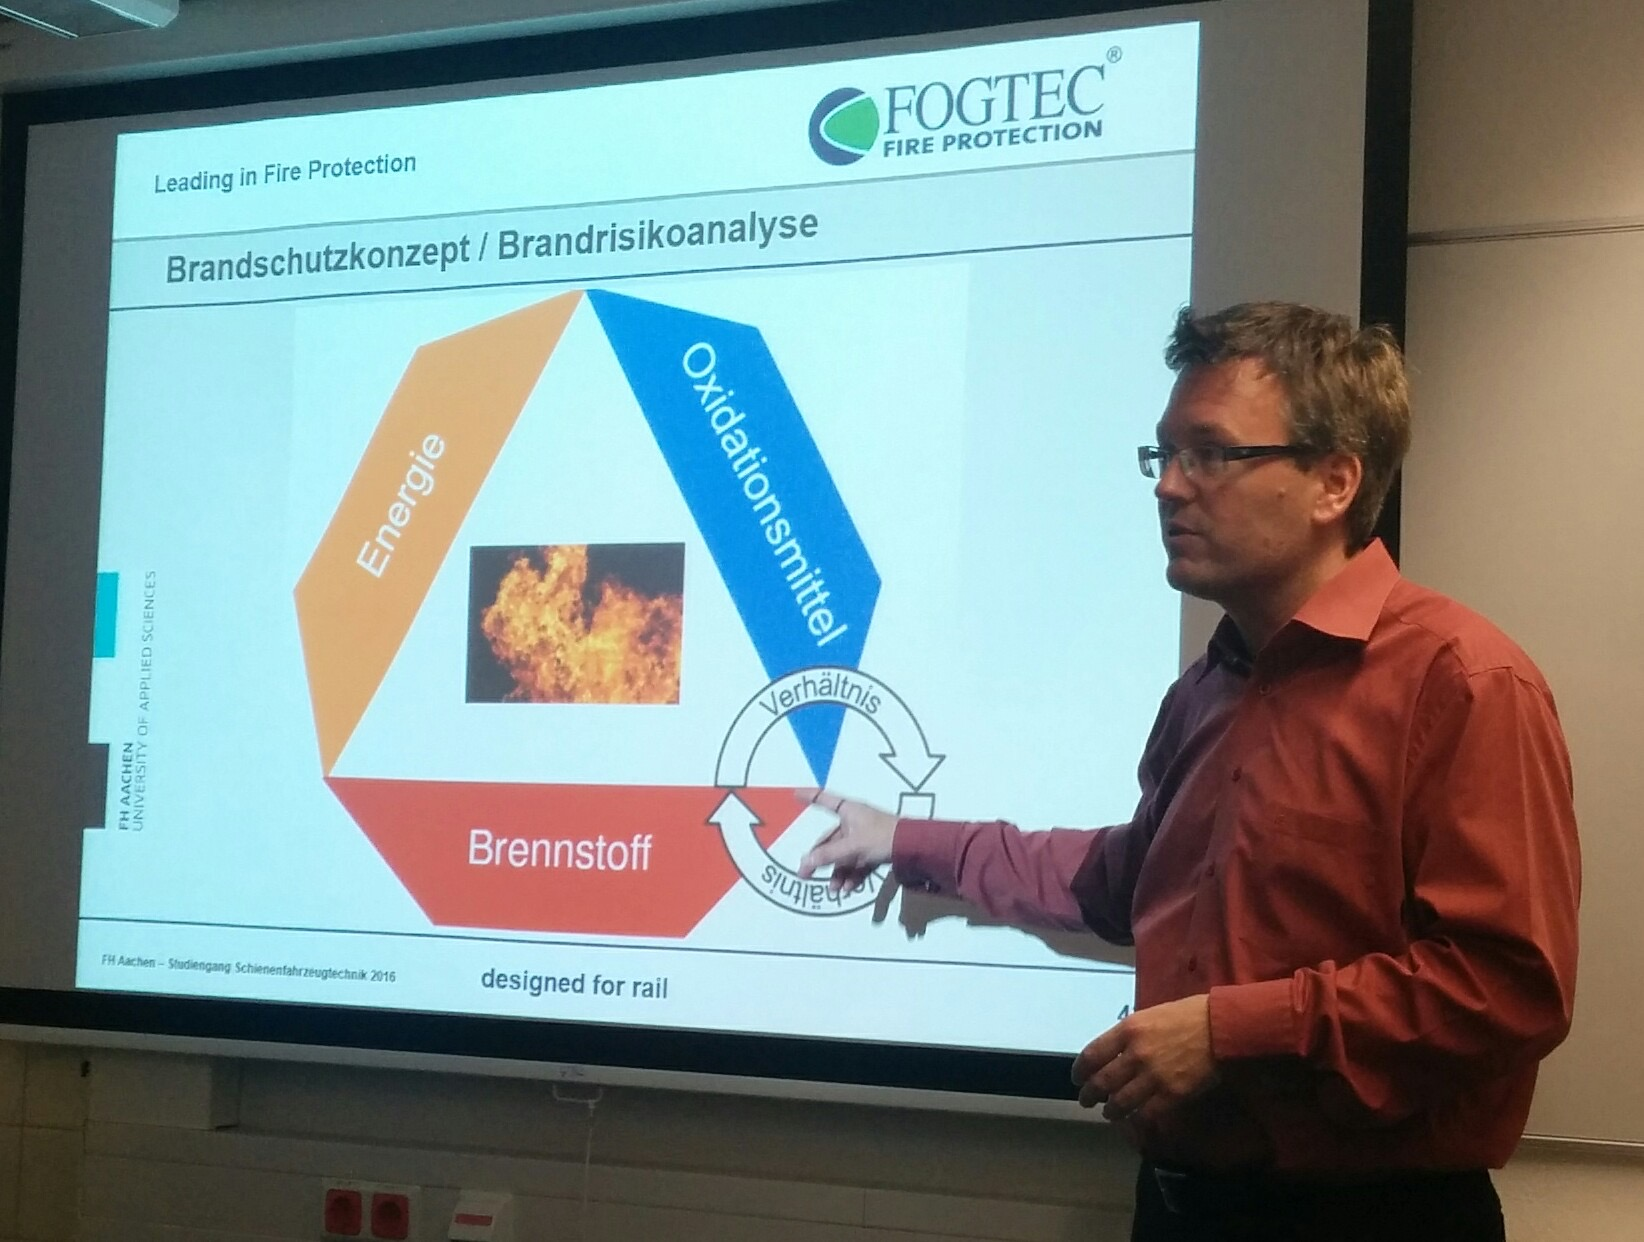
\includegraphics[width = 5cm]{Roger}};
%\node at (0,1) {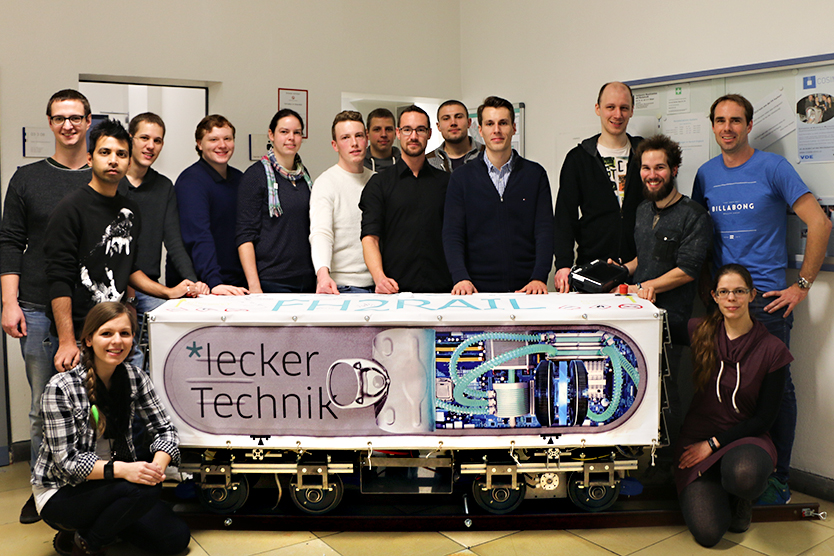
\includegraphics[width = 6cm]{Team}};
%\node at (-1,-2) {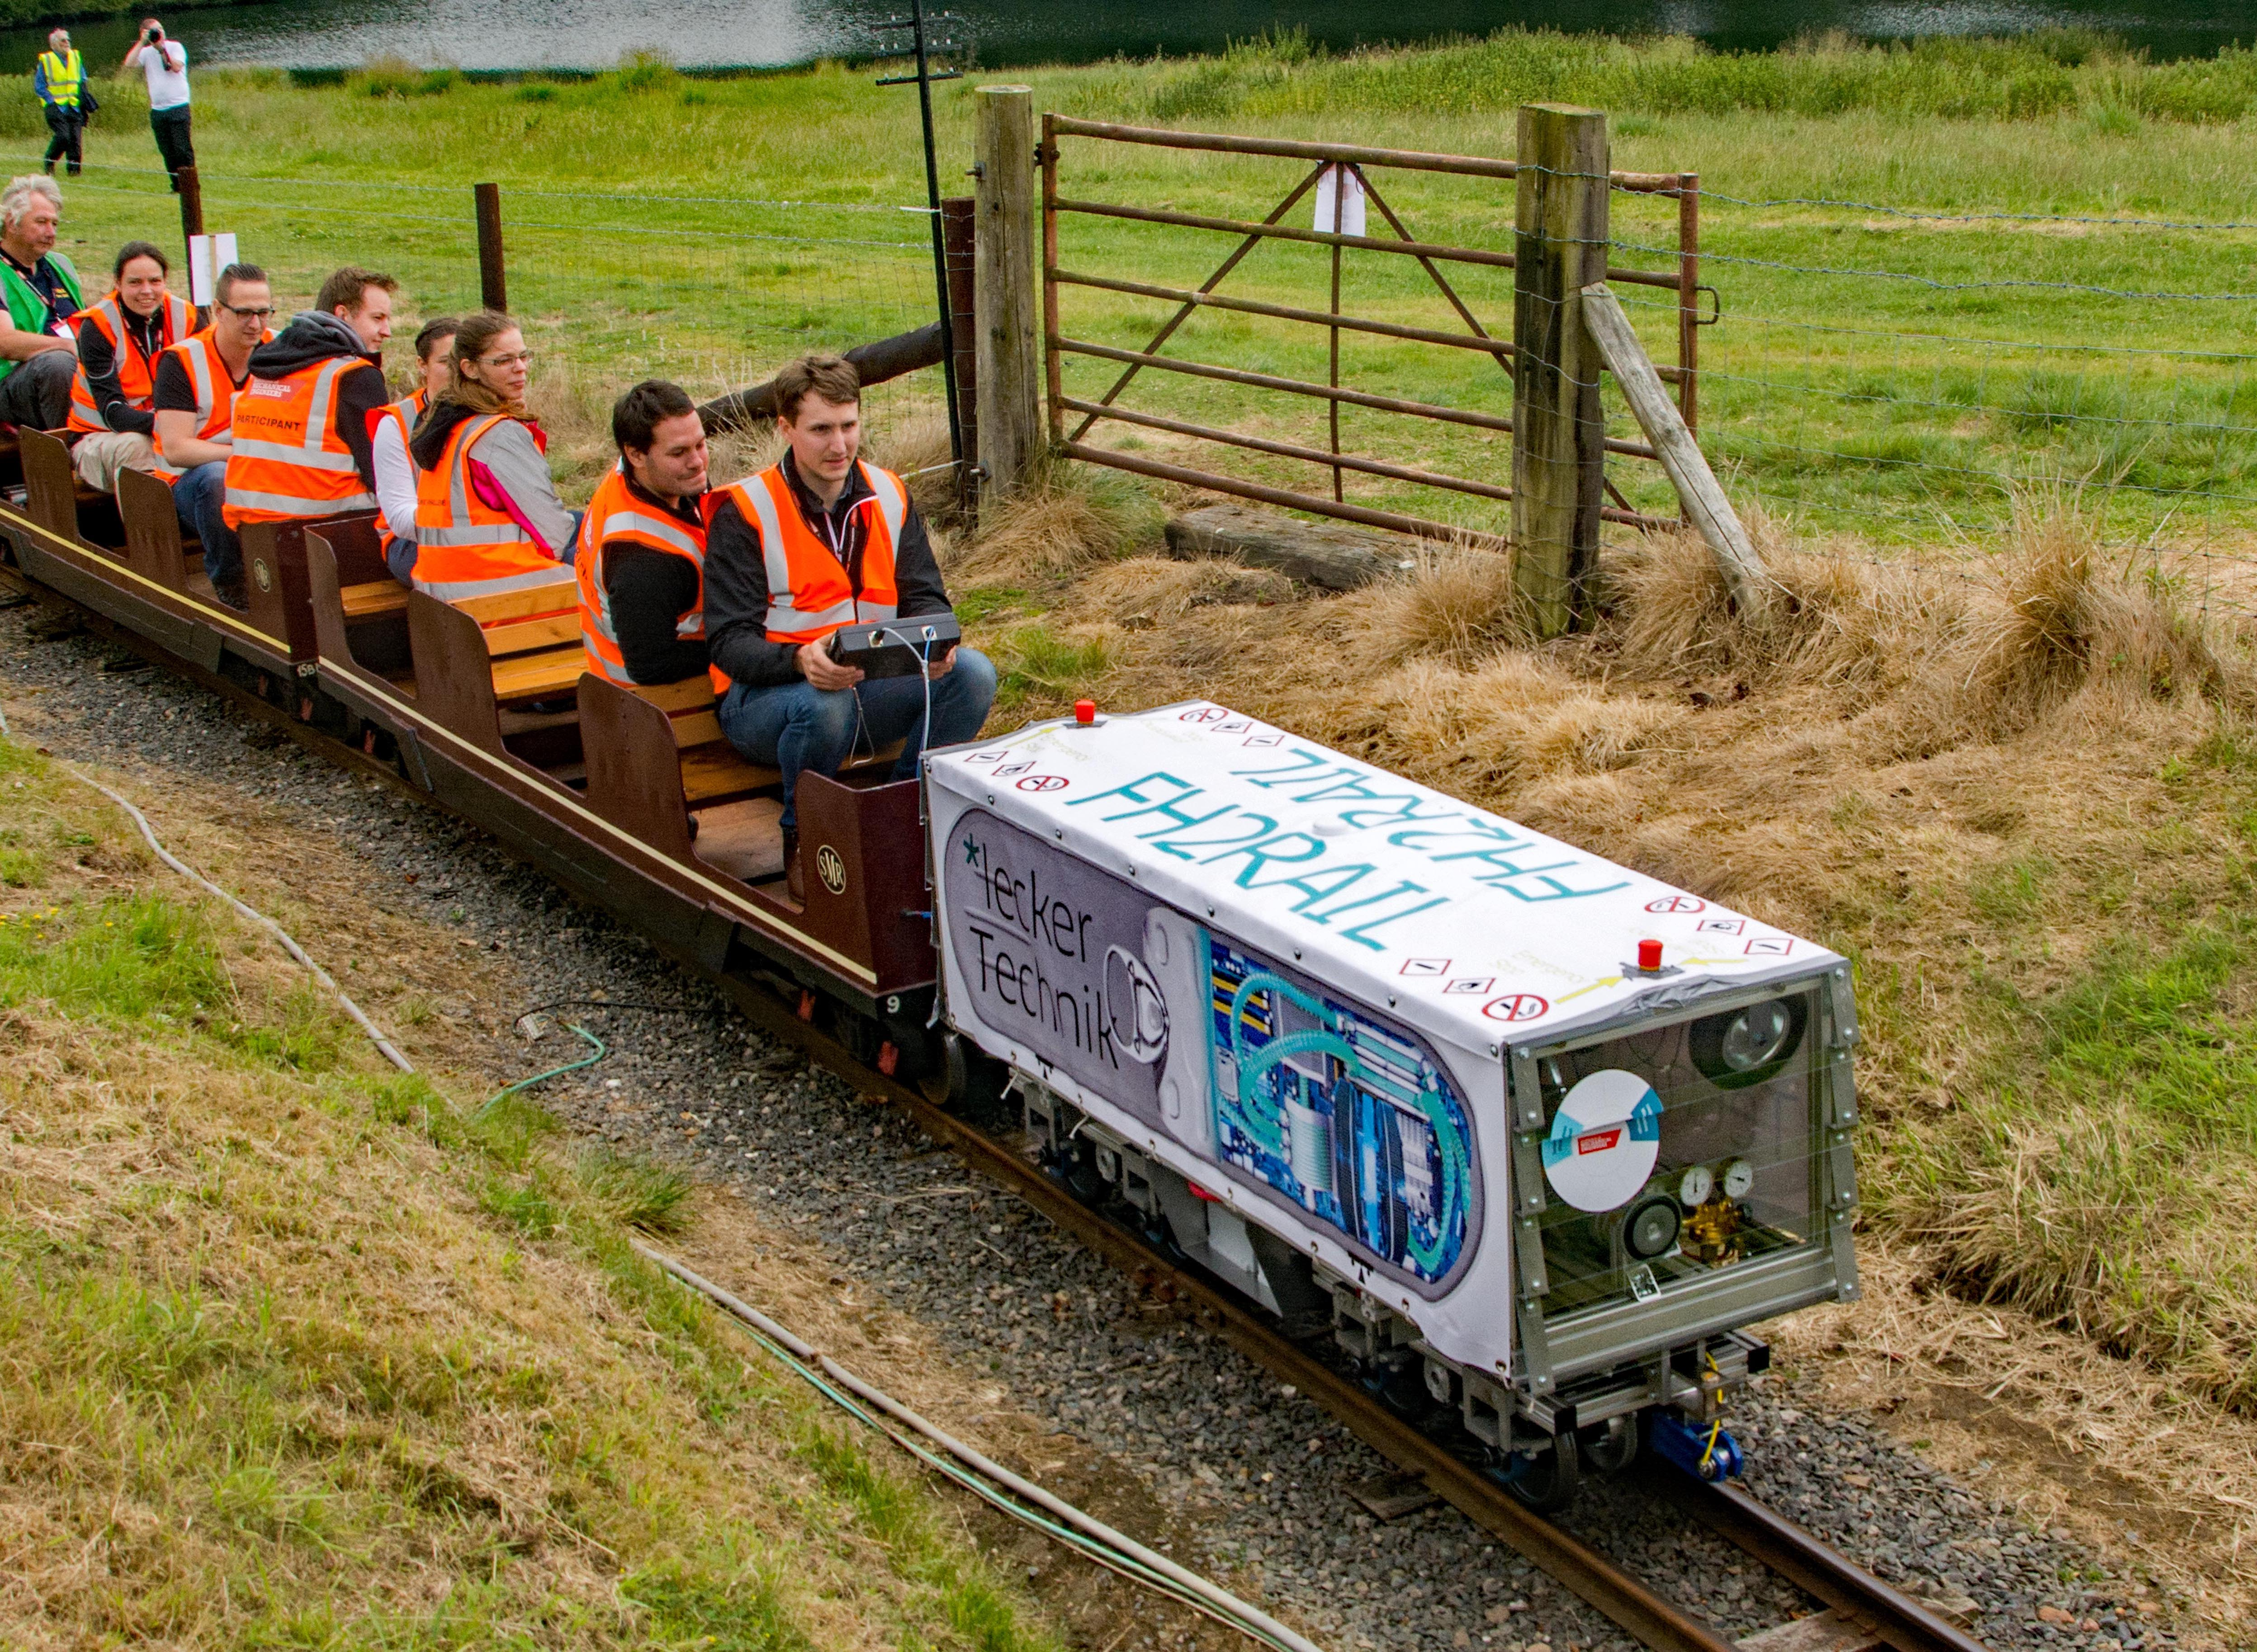
\includegraphics[width = 6cm]{TrainEmma}};
%
%\node at (4,-2) {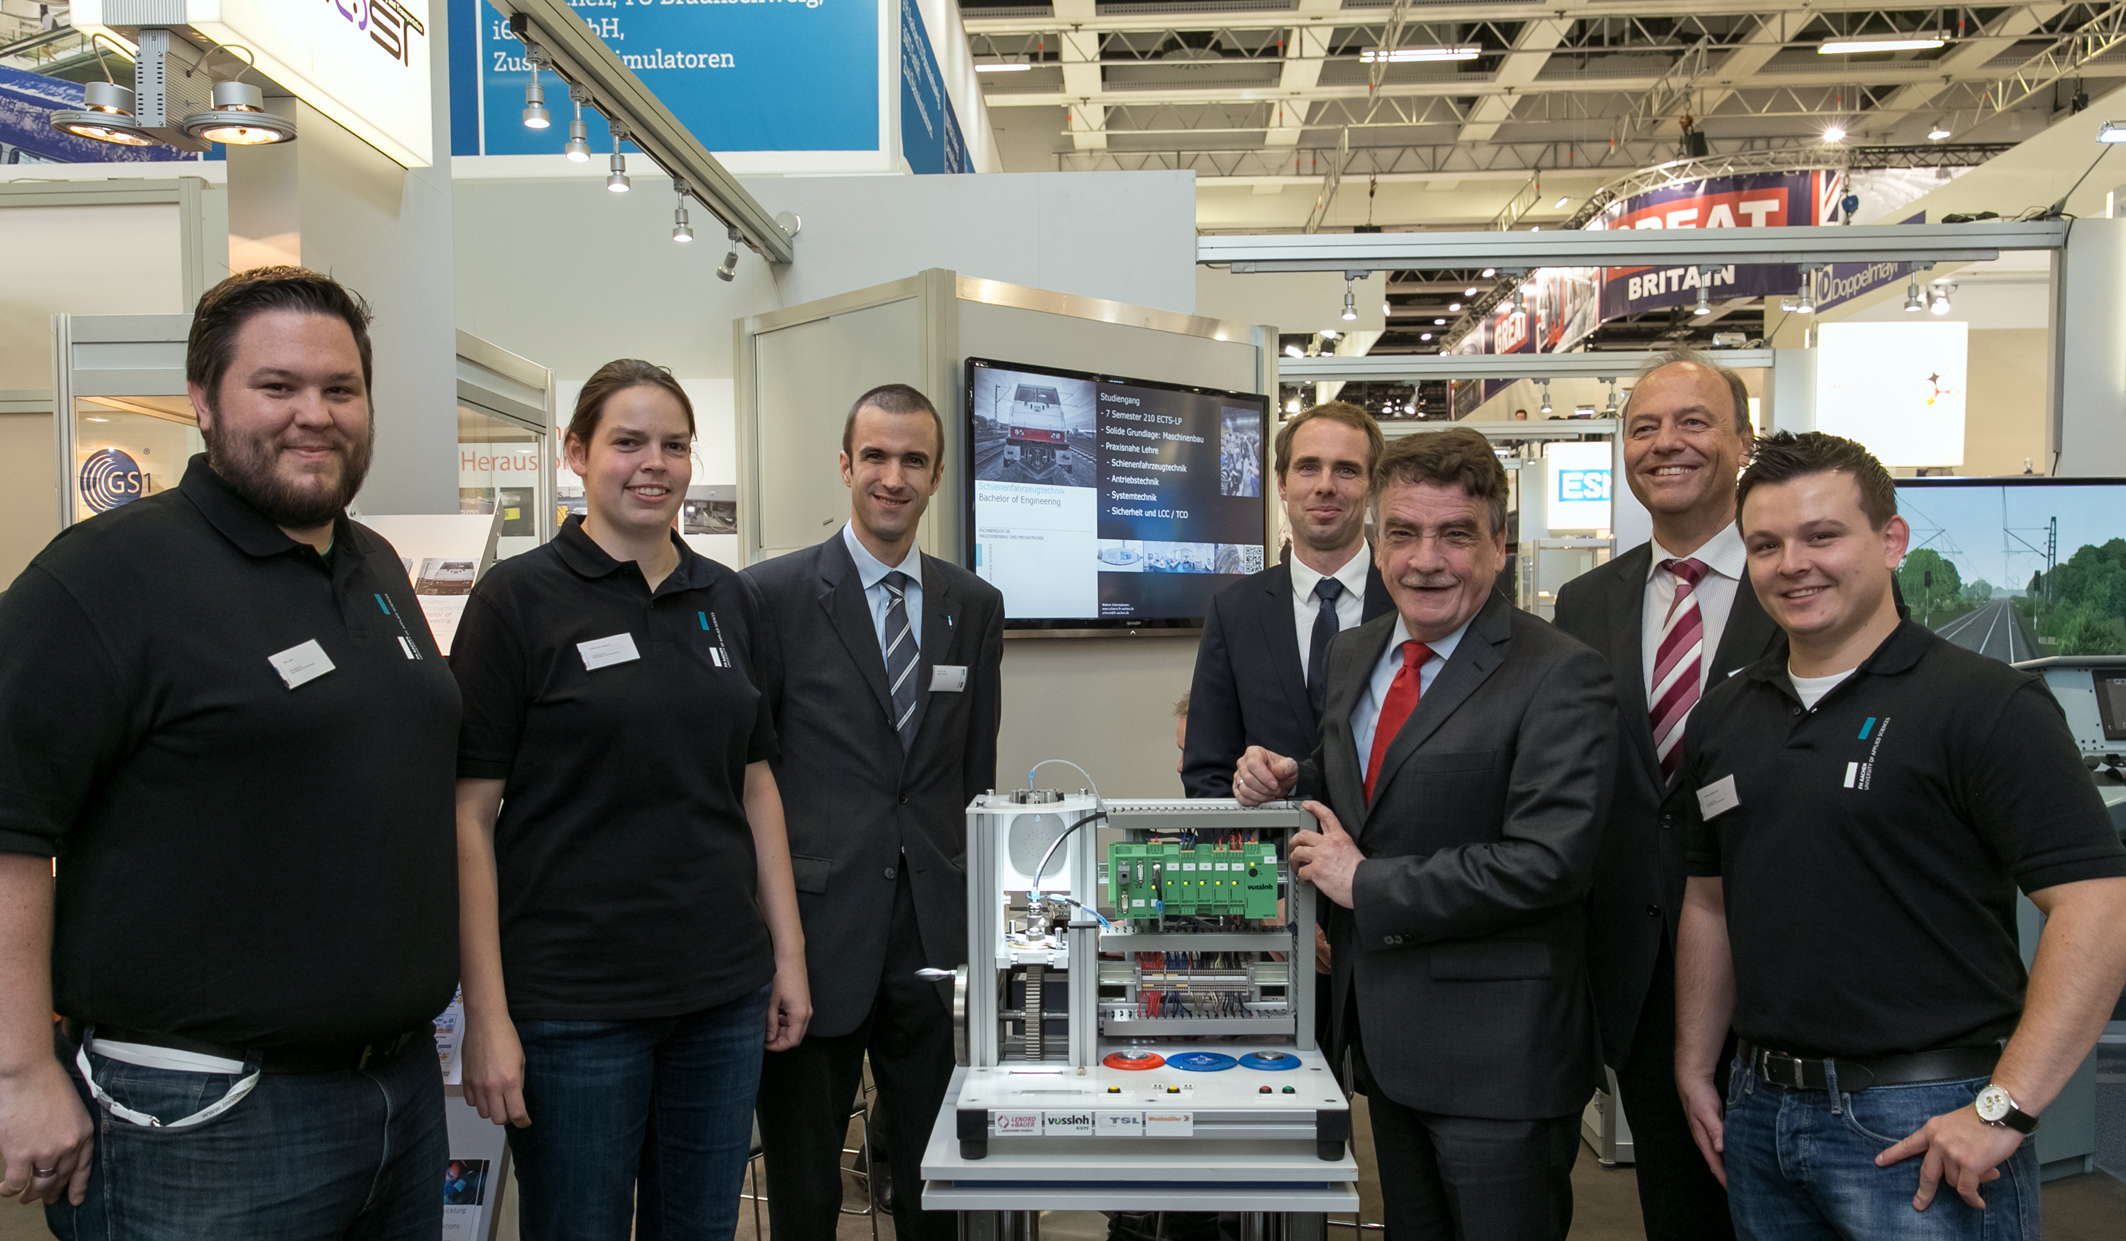
\includegraphics[width = 5cm]{InnotransStudis}};
%
%\end{tikzpicture}
%\end{center}
%}
%
%\frame{\frametitle{Was wir tun}
%\framesubtitle{Lehre, Forschung, Entwickung und Beratung entlang des Lebenszyklus im Bahnverkehr}
%\begin{columns}[t] 
%     \begin{column}[T]{7cm} 
%     	\begin{itemize}
%     		\only<1>{\item Lehre:
%		\begin{itemize}
%		\item Schienenfahrzeugtechnik
%		\begin{itemize}
%		\item Mechanisches Subsystem
%		\end{itemize}
%		\item Bahnantriebe
%		\begin{itemize}
%		\item Elektrische Antriebe
%		\item Diesel- und hybride Antriebe
%		\end{itemize}
%		\item Leit- und Sicherungstechnik
%		\item Steuerungs- und Simulationstechnik
%		\item Herstellung und Vermarktung
%		\item Antriebstechnik
%		\begin{itemize}
%		\item Elektrische Antriebe
%		\item Fluidtechnik
%		\end{itemize}
%		\item Statistische Methoden
%		\item Methoden des QM
%		\end{itemize}}
%		\only<2->{\item Current R\&D foci:
%		\begin{itemize}
%		\item IoT-connected wagon ``Wagon 4.0''
%		\item Refurbishment of legacy electrical locomotives
%		\item Reliability Estimation using Big Data approaches
%		\item Usage of Additive Manufacturing 
%		\item Wheel-Rail-Contact Modelling% under sanding
%		\item Ad hoc-Estimation of braking curves
%		\item Applications of machine learning for railways  
%		\end{itemize}}
%     	\end{itemize}
%     \end{column}
%     	\begin{column}[T]{7cm} 
%         	\begin{center}
%            		\only<1>{\includegraphics[width=0.8\textwidth]{Lehre}\source{}}
%			%%
%			\only<2>{\includegraphics[width=0.95\textwidth]{TrainConceptWagon40}\source{}}
%			\only<3>{\includegraphics[width=0.7\textwidth]{Rekuperation}\source{}}
%			%%
%			\only<4>{
%			\vspace{-.6cm}
%			\begin{tikzpicture}
%                            \begin{axis}[no marks,
%                            xmax=15, xmin = 0,
%                             ymin = 0, ymax = 1, grid=both,
%                            %axis lines=middle, 
%                            %ylabel = {$p$},
%                            xlabel = {$t/\mathrm{a}$},
%                            legend entries={$\bar{F}$, $h$, $\bar{F}_{\text{main}}$, $\hat{F}$, 
%                            $\hat{h}$}, 
%                            legend style = {at={(0.05,0.5)},
%                                    anchor=west}]
%                            
%                              \addplot[thick, draw = magenta!70!black] table[x=t,y=Fq] {WeibullEstCensored.dat}; 
%                            
%                             \addplot[thick, draw = orange!80!black] table[x=t,y=h] {WeibullEstCensored.dat}; 
%                            
%                             \addplot[thick, draw = red!70!black] table[x=t,y=Fqest] {WeibullEstCensored2.dat}; 
%                                
%                              
%                              \addplot[thick, draw = green!70!black] table[x=t,y=Fqsim] {WeibullEstCensored.dat}; 
%                              
%                              
%                             \addplot[thick, draw = blue!70!black] table[x=t,y=hest] {WeibullEstCensored.dat}
%                             coordinate [pos=0.5] (A)
%                               coordinate [pos=0.6]  (B)
%                             ; 
%                             \fill[fill = blue!70!black, opacity = .7] (A) -| (B)
%                             node [pos=0.75,anchor=west]
%                                 {$\triangle h$};
%                             \end{axis}
%                            \end{tikzpicture}
%                            }
%                            \only<5>{\includegraphics[width=0.2\textwidth]{TestFeder4b} \hspace{3mm}
%                            		\includegraphics[width=0.2\textwidth]{TestFeder4a} \vspace{3mm}\\
%					\includegraphics[width=0.2\textwidth]{TestFeder1b}\hspace{3mm}
%					\includegraphics[width=0.4\textwidth]{TestFeder1a}}
%                            \only<6>{\includegraphics[width=0.9\textwidth]{AreaComp}\source{}}
%                            \only<7>{\vspace{-.6cm}
%                            \includegraphics[width=0.7\textwidth]{ETCSmhist}\\
%                            		\hspace{1.5cm} \includegraphics[width=0.7\textwidth]{ETCShist}}
%		\only<8>{\includegraphics[width=0.9\textwidth]{170505GPCascadeClassifier}}
%        		\end{center}
%     \end{column}
% \end{columns}
%}

{
\usebackgroundtemplate{\includegraphics[width= \paperwidth]{DualesStudium.jpg}}

\section{Dualer Studiengang BEng Schienenfahrzeugtechnik}
\frame{\vspace{1.5cm}

\begin{center}
 \color{white} \usebeamerfont{title}{Studiengang BEng Schienenfahrzeugtechnik\\
 DI Rail - Duale Ingenieurausbildung Schienenfahrzeugtechnik}
\end{center}
}
}

\frame{\frametitle{Ein Studiengang - drei Studienmodelle}
\framesubtitle{}
\begin{columns}[t] 
     \begin{column}[T]{6cm} 
     	\begin{itemize}
     		\item Vollzeit
		\begin{itemize}
		\item 7 Semester
		\end{itemize}
		\item Ausbildungsintegriert dual
		\begin{itemize}
		\item 9 oder 11 Semester
		\item Abh\"angig von der Form des Vertiefungsstudiums (Vollzeit/Teilzeit)
		\end{itemize}
		\item Teilzeit
		\begin{itemize}
		\item 11 Semester
		\end{itemize}
     	\end{itemize}
     \end{column}
     	\begin{column}[T]{6cm} 
         	\begin{center}
            		\includegraphics[width=0.9\textwidth]{Studienverlauf}\source{}
        		\end{center}
     \end{column}
 \end{columns}
}

\frame{\frametitle{Duales Studium: das Krefelder Modell}
\framesubtitle{}
\begin{columns}[t] 
     \begin{column}[T]{6cm} 
     	\begin{itemize}
     		\item Duale Ausbildung an drei Tagen im Unternehmen, z.B.
		\begin{itemize}
		\item Mechatroniker(in)
		\item Zerspanungsmechaniker(in)
		\item Eisenbahner(in) im Betriebsdienst
		\end{itemize}
		\item Berufsschule entf\"allt
		\item IHK-Abschluss nach zwei Jahren
     	\end{itemize}
     \end{column}
     	\begin{column}[T]{8cm} 
         	\begin{center}
            		\begin{tikzpicture}[
                    %scale = 0.5,
                    studrect/.style={rectangle,align = center, 
                    draw = mint!75!black, 
                    fill =mint!75!black, opacity = 0.7, minimum width = 2.9cm, minimum height = 0.9cm, rounded corners}, 
                    veearr/.style={>=stealth, ->,line width = 6, draw = gray, opacity = 1}, 
                    dayrect/.style={rectangle, align = center, 
                    draw = gray!30, 
                    fill =gray!30, opacity = 0.7, rounded corners, minimum height = 6.3cm, minimum width = 1.3cm},
                    modarr/.style={>=stealth, ->,line width = 3, draw = gray, opacity = 1},
                    workrect/.style={rectangle,align = center, 
                    draw = gray!50, 
                    fill =gray!50, opacity = 0.7, minimum width = 4.4cm, minimum height = 0.9cm, rounded corners},
                    otrect/.style={rectangle,align = center, 
                    draw = gray!50, 
                    fill =gray!50, opacity = 0.7, minimum width = 7.5cm, minimum height = 0.3cm, rounded corners},  
                    node distance = 1cm]
                    
                    \node[dayrect] at (0,-1) {};
                    \node at (0,1.5) {Mo};
                    
                    \node[dayrect] at (1.5,-1) {};
                    \node at (1.5,1.5) {Di};
                    \node[dayrect] at (3,-1) {};
                    \node at (3,1.5) {Mi};
                    \node[dayrect] at (4.5,-1) {};
                    \node at (4.5,1.5) {Do};
                    \node[dayrect] at (6,-1) {};
                    \node at (6,1.5) {Fr};
                     \node[studrect] at (5.25,.6) {1. Semester};
                    \node[workrect] at (1.5,.6) {Unternehmen};
		   \node[otrect] at (3,-.1) {};
                    \node[studrect] at (0.75,-.8) {2. Semester};
                    \node[workrect] at (4.5,-.8) {Unternehmen};
                    \node[otrect] at (3,-1.5) {};
                    \node[studrect] at (0.75,-2.2) {3. Semester};
                    \node[workrect] at (4.5,-2.2) {Unternehmen};
                    \node[otrect] at (3,-2.9) {};

                    \node[studrect] at (5.25,-3.6) {4. Semester};
                    \node[workrect] at (1.5,-3.6) {Unternehmen};
                    \end{tikzpicture}
        		\end{center}
     \end{column}
 \end{columns}
}

\frame{\frametitle{Struktur des Studiengangs - Basisstudium}
\framesubtitle{}
\tikzset{font=\small}
%\begin{center}
\begin{tikzpicture}[
scale = 0.5,
modrect/.style={rectangle,align = center, 
draw = mint!75!black, 
fill =mint!75!black, opacity = 0.7, minimum width = 2.5cm, minimum height = .95cm, rounded corners}, 
veearr/.style={>=stealth, ->,line width = 6, draw = gray, opacity = 1}, 
semrect/.style={rectangle, align = center, 
draw = gray!50, 
fill =gray!50, opacity = 0.7, rounded corners, minimum height = 7.5cm, minimum width = 2.7cm},
modarr/.style={>=stealth, ->,line width = 3, draw = gray, opacity = 1}, 
node distance = 1.05cm]

\node[semrect] at (-11,-8.2) {};
\node (1) at (-11,-2) {1. Semester };
\node [modrect, below of = 1, draw] (M1) {Mathematik 1};
\node[modrect, below of = M1, draw]  (TM1) {Technische \\Mechanik 1};
\node[modrect, below of = TM1, draw]  (Ph) {Physik};
\node[modrect, below of = Ph, draw]  (WK) {Werkstoffkunde};
\node[modrect, below of = WK, draw]  (TZ) {CAD/Techn.\\Zeichnen}; 

\node[semrect] at (0,-8.2) {};
\node (2) at (0,-2) {2. Semester };
\node [modrect, below of = 2, draw] (M2) {Mathematik 2};
\node[modrect, below of = M2, draw]  (TM2) {Technische \\Mechanik 2};
\node[modrect, below of = TM2, draw]  (FV) {Technisches\\Englisch};
\node[modrect, below of = FV, draw]  (DV) {Daten-\\verarbeitung};
\node[modrect, below of = DV, draw]  (ET) {Elektrotechnik\\Elektronik};

\node[semrect] at (11,-8.2) {};
\node (3) at (11,-2) {3. Semester };
\node [modrect, below of = 3, draw] (M3) {Mathematik 3};
\node[modrect, below of = M3, draw]  (TM3) {Technische \\Mechanik 3};
\node[modrect, below of = TM3, draw]  (KE) {Konstruktions-\\elemente 1};
\node[modrect, below of = KE, draw]  (SRT) {Fertigungs-\\verfahren 1};
\node[modrect, below of = SRT, draw]  (TD) {Thermo-\\dynamik};
\node[modrect, below of = TD, draw]  (BW) {Allgemeine\\Kompetenzen};

\end{tikzpicture}
%\end{center}
}



\frame{\frametitle{Struktur des Studiengangs - Basisstudium dual}
\framesubtitle{}
\tikzset{font=\small}
%\begin{center}
\begin{tikzpicture}[
scale = 0.5,
modrect/.style={rectangle,align = center, 
draw = mint!75!black, 
fill =mint!75!black, opacity = 0.7, minimum width = 2.5cm, minimum height = .95cm, rounded corners}, 
veearr/.style={>=stealth, ->,line width = 6, draw = gray, opacity = 1}, 
semrect/.style={rectangle, align = center, 
draw = gray!50, 
fill =gray!50, opacity = 0.7, rounded corners, minimum height = 7.2cm, minimum width = 2.7cm},
modarr/.style={>=stealth, ->,line width = 3, draw = gray, opacity = 1}, 
node distance = 1.05cm]

\node[semrect] at (-11,-8.2) {};
\node (1) at (-11,-1.7) {1. Semester };
\node [modrect, below of = 1, draw] (M1) {Mathematik 1};
\node[modrect, below of = M1, draw]  (TM1) {Technische\\Mechanik 1};
%\node[modrect, below of = TM1, draw]  (Ph) {Physik};
%\node[modrect, below of = Ph, draw]  (WK) {Werkstoffkunde};
%\node[modrect, below of = WK, draw]  (TZ) {CAD/Techn.\\Zeichnen}; 

\node[semrect] at (-5.5,-8.2) {};
\node (2) at (-5.5,-1.7) {2. Semester };


\node[semrect] at (0,-8.2) {};
\node (3) at (0,-1.7) {3. Semester };
\node [modrect, below of = 2, draw] (M2) {Mathematik 2};
\node[modrect, below of = M2, draw]  (TM2) {Daten-\\verarbeitung};
\node[modrect, below of = TM2, draw]  (FV) {Technisches\\Englisch};
%\node[modrect, below of = FV, draw]  (DV) {Daten-\\verarbeitung};
%\node[modrect, below of = DV, draw]  (ET) {Elektrotechnik\\Elektronik};
\node [modrect, below of = 3, draw = none, fill = none] (M1) {};
\node[modrect, below of = M1, draw = none, fill = none]  (TM1) {};
\node[modrect, below of = TM1, draw]  (Ph) {Physik};
\node[modrect, below of = Ph, draw]  (WK) {Werkstoffkunde};
\node[modrect, below of = WK, draw]  (TZ) {CAD/Techn.\\Zeichnen}; 

\node[semrect] at (5.5,-8.2) {};
\node (4) at (5.5,-1.7) {4. Semester};
\node [modrect, below of = 4, draw= none, fill = none] (M2) {};
\node[modrect, below of = M2, draw= none, fill = none]  (TM2) {};
\node[modrect, below of = TM2, draw=none, fill = none]  (FV) {};
\node[modrect, below of = FV, draw]  (DV) {Informations-\\technik 1};
\node[modrect, below of = DV, draw]  (ET) {Elektrotechnik\\Elektronik};
\node[modrect, below of = ET, draw]  (Pro) {Projekt 1};

\node[semrect] at (11,-8.2) {};
\node (5) at (11,-1.7) {5. Semester};
\node [modrect, below of = 5, draw] (M3) {Mathematik 3};
\node[modrect, below of = M3, draw]  (TM3) {Technische \\Mechanik 3};
\node[modrect, below of = TM3, draw]  (KE) {Konstruktions-\\elemente 1};
\node[modrect, below of = KE, draw]  (SRT) {Fertigungs-\\verfahren 1};
\node[modrect, below of = SRT, draw]  (TD) {Thermo-\\dynamik};
\node[modrect, below of = TD, draw]  (BW) {Allgemeine\\Kompetenzen};


\end{tikzpicture}
%\end{center}
}

\frame{\frametitle{Struktur des Studiengangs - Vertiefungsstudium}
\framesubtitle{}
\begin{center}
\tikzset{font=\small}
\begin{tikzpicture}[
scale = 0.5,
modrect/.style={rectangle,align = center, 
draw = mint!75!black, 
fill =mint!75!black, opacity = 0.7, minimum width = 3cm, minimum height = .95cm, rounded corners}, 
veearr/.style={>=stealth, ->,line width = 6, draw = gray, opacity = 1}, 
semrect/.style={rectangle, align = center, 
draw = gray!50, 
fill =gray!50, opacity = 0.7, rounded corners, minimum height = 7.5cm, minimum width = 3.1cm},
modarr/.style={>=stealth, ->,line width = 3, draw = gray, opacity = 1}, 
node distance = 1.05cm]



\node[semrect] at (0,1) {};
\node (6) at (0,7.8) {6. Semester };
\node [modrect, below of = 6, draw] (SFT1) {Betriebswirtschaft\\und Technik};
\node[modrect, below of = SFT1, draw]  (SFA1) {Regelungs-\\technik};
\node[modrect, below of = SFA1, draw]  (KE2) {Konstruktions-\\elemente 2};
\node[modrect, below of = KE2, draw]  (LST) {Str\"omungs-\\lehre};
\node[modrect, below of = LST, draw]  (Eng) {Thermodynamik};
\node[modrect, below of = Eng, draw,]  (QSS) {Schienenfahrzeug-\\antriebe 1};

\node[semrect] at (7,1) {};
\node (7) at (7,7.8) {7. Semester };
\node [modrect, below of = 7, draw] (V1) {Herstellung und\\Vermarktung};
\node[modrect, below of = V1, draw]  (V2) {Qualit\"at und\\Sicherheit};
\node[modrect, below of = V2, draw]  (V3) {Schienenfahrzeug-\\technik 1};
\node[modrect, below of = V3, draw]  (V4) {Leit- und\\Sicherungst.};
\node[modrect, below of = V4, draw]  (V5) {Allgemeine\\Kompetenzen};

\node[semrect] at (14,1) {};
\node (8) at (14,7.8) {8. Semester };
\node [modrect, below of = 8, draw] (SFT2) {Schienenfahrzeug-\\technik 2};
\node[modrect, below of = SFT2, draw]  (SFA2) {Schienenfahrzeug-\\antriebe 2};
\node[modrect, below of = SFA2, draw]  (HuV) {Wahlmodul};
\node[modrect, below of = HuV, draw]  (SSS) {Steuerung und\\ Simulation};
\node[modrect, below of = SSS, draw]  (WM3) {Projekt 2};
%\node[modrect, below of = WM3, draw]  (WM4) {Wahlmodul};


\node[semrect] at (21,1) {};
\node (9) at (21,7.8) {9. Semester };
\node[modrect, below of = 9, draw] (P) {Praxisphase\\ (12 Wochen)};
\node[modrect, below of = P, draw]  (B) {Bachelorarbeit\\(9 Wochen)};
\node[modrect, below of = B, draw]  (B) {Kolloquium};
\end{tikzpicture}
\end{center}
}

\frame{\frametitle{Vorteile f\"ur Unternehmen und duale Azubis}
\framesubtitle{}
\begin{columns}[t] 
     \begin{column}[T]{7cm} 
     \textbf{Unternehmen:}
     	\begin{itemize}
     		\item Fr\"uhe Rekrutierung
		\item Hervorragend qualifizierte Bewerber
		\item Langfristige Bindung
		\item Fachspezifisches Studium
		\item Unternehmenserfahrung
     	\end{itemize}
     \end{column}
     	\begin{column}[T]{7cm} 
	\textbf{Azubis:}
         	\begin{itemize}
		\item Studienfinanzierung
		\item Motivation f\"ur Studium durch T\"atigkeit in der Wirtschaft
		\item Netzwerkaufbau bereits im Studium
		\item Praxiserfahrung
		\end{itemize}
     \end{column}
 \end{columns}
 \begin{center}
 \href{https://www.youtube.com/watch?v=bTGwHGsTZJU}{\includegraphics[width= 5cm]{DualesStudium.jpg}\\Klicken f\"ur Image-Video}
 \end{center}
}

\frame{\frametitle{Bei Interesse: weitere Schritte}
\framesubtitle{}
\begin{itemize}
\item[$\square$] Unterzeichnung Kooperationsvertrag
\item[$\square$] LoI zur Kapazit\"atsplanung
\item[$\square$] Abstimmung mit lokaler IHK - begleitet durch FH-Beauftragten A. Beumers
\item[$\square$] Ggf. Unterst\"utzung bei Marketing und Auswahl
\end{itemize}
\vspace{2cm}

Kontakt:\\
Prof. Dr. Raphael Pfaff\\
pfaff@fh-aachen.de\\
+49-151-70052454
}


%\frame{\frametitle{RVE Basic Modules}
%\framesubtitle{}
%\begin{columns}[t] 
%     \begin{column}[T]{7cm} 
%     \textbf{Economy and Technology} (5 credits)
%     	\begin{itemize}
%		\item Ecomomics:
%		\begin{itemize}
%     		\item Basic Concepts
%		\item Economic Systems
%		\item Market and State
%		\item Legal forms and frameworks
%		\item Profit and Loss of RUs
%		\item Environment
%		\end{itemize}
%		\item Basic Rail Vehicle Technology
%		\item Mass-Transit-Applications
%		\item Introduction to Signaling Systems
%		\item Introduction to Drives
%		\item Basics of Lifecycle Costing
%     	\end{itemize}
%     \end{column}
%     	\begin{column}[T]{7cm} 
%	\textbf{Quality and Safety in the Lifecycle} (5 credits)
%         	\begin{itemize}
%     		\item Maintenance
%		\begin{itemize}
%		\item Planning
%		\item Infrastructure
%		\item Execution
%		\item Lifecycle cost modelling and optimisation
%		\end{itemize}
%		\item Safety
%		\begin{itemize}
%		\item Reliability and Safety Engineering
%		\item Risk assessment
%		\item Risk reduction
%		\item Homologation process
%		\end{itemize}
%	     	\end{itemize}
%     \end{column}
% \end{columns}
%}
%
%
%\frame{\frametitle{RVE Core Modules: Rail Vehicle Engineering}
%\framesubtitle{}
%\begin{columns}[t] 
%     \begin{column}[T]{7cm} 
%     \textbf{Rail Vehicle Engineering 1} (5 credits)
%     	\begin{itemize}
%     		\item Introduction to Rail Vehicles
%		\begin{itemize}
%		\item Taxonomy
%		\item Requirements
%		\item Structures
%		\end{itemize}
%		\item Running dynamics of rail vehciles
%		\begin{itemize}
%		\item Longitudinal dynamics
%		\item Lateral dynamics
%		\item Wheel rail interface
%		\end{itemize}
%		\item Vehicle design
%		\begin{itemize}
%		\item Principles
%		\item Gauging
%		\end{itemize}
%		\item Running gear
%     	\end{itemize}
%     \end{column}
%     	\begin{column}[T]{7cm} 
%	\textbf{Rail Vehicle Engineering 2} (5 credits)
%         	\begin{itemize}
%     		\item Running dynamics and comfort
%%		\begin{itemize}
%%		\item Stability of vehicles
%%		\item Comfort dynamics
%%		\end{itemize}
%		\item Vehicle types and components
%%		\begin{itemize}
%%		\item Passenger vehicles
%%		\item Freight vehicles
%%		\end{itemize}
%		\item Human-Machine Interface
%		\item Safety in Rail Vehicles
%		\item Buff and Draft Gear
%		\item Railway Braking System
%		\begin{itemize}
%		\item Automatic Brake
%		\item Brake force generation
%		\item Compressed air supply
%		\item Driver's Brake Valve
%		\item ep-Brake, Emergency Brake
%		\item Wheel-Slide-Protection
%		\item Operational Aspects
%		\end{itemize}
%     	\end{itemize}
%     \end{column}
% \end{columns}
%}
%
%\frame{\frametitle{RVE Core Modules: Drives}
%\framesubtitle{}
%\begin{columns}[t] 
%     \begin{column}[T]{7cm} 
%     \textbf{Electrical Rail Vehicle Drives 1} (5 credits)
%     	\begin{itemize}
%     		\item Tractive forces
%		\item Running resistances
%		\item Drive Train dynamics
%		\item Power Collection
%		\item Power Transformer
%		\item Converters
%		\item Electrical Motors
%		\begin{itemize}
%		\item Characteristics
%		\item Control system
%		\end{itemize}
%		\item Gear system
%		\item Wheel Slip Prevention
%     	\end{itemize}
%     \end{column}
%     	\begin{column}[T]{7cm} 
%	\textbf{Diesel and Hybrid Rail Vehicle Drives 2} (5 credits)
%         	\begin{itemize}
%     		\item Diesel Engines
%		\begin{itemize}
%		\item Design principles
%		\item Power conversion
%		\item Efficiency
%		\item Adjustment
%		\item Maintenance
%		\end{itemize}
%		\item Diesel-Electric Drivetrain
%		\begin{itemize}
%		\item Generators and Converters
%		\end{itemize}
%		\item Diesel-Hydraulic Drivetrain
%		\begin{itemize}
%		\item Design Principles
%		\item Power Conversion
%		\end{itemize}
%		\item Energy Storage
%		\begin{itemize}
%		\item Battery Systems
%		\item Battery Management
%		\end{itemize}
%     	\end{itemize}
%     \end{column}
% \end{columns}
%}
%
%\frame{\frametitle{RVE Core Modules: Rail Systems Engineering}
%\framesubtitle{}
%\begin{columns}[t] 
%     \begin{column}[T]{7cm} 
%     \textbf{Signalling and Interlock} (5 credits)
%     	\begin{itemize}
%     		\item Signal types
%		\item Block signalling
%		\item Train Protection Systems
%		\begin{itemize}
%		\item Intermittent TPS (PZB)
%		\item Continuous Train Control (LZB)
%		\item European Train Control System (ETCS)
%		\end{itemize}
%		\item Cab signalling
%		\item Interlocking architecture
%     	\end{itemize}
%     \end{column}
%     	\begin{column}[T]{7cm} 
%	\textbf{Control and Simulation Techniques} (5 credits)
%         	\begin{itemize}
%     		\item Control Systems for Rail Vehicles
%		\begin{itemize}
%		\item Requirements
%		\item Architectures
%		\item Bus communication (MVB, WTB, CAN, ...)
%		\item Documentation
%		\item Testing
%		\end{itemize}
%		\item Simulation and control applications
%		\begin{itemize}
%		\item Impact simulation
%		\item Door control system
%		\end{itemize}
%		\end{itemize}
%	\end{column}
%     	 \end{columns}
%}
%
%\frame{\frametitle{RVE Additional Modules}
%\framesubtitle{}
%\begin{columns}[t] 
%     \begin{column}[T]{7cm} 
%     \textbf{Manufacturing and Marketing of Rail Vehicles} (5 credits)
%     	\begin{itemize}
%     		\item Market segmentation
%		\item Market barriers
%		\item Contract design
%		\item Requirements Engineering
%		\item Project estimation
%		\item Project planning
%		\item Rail Vehicle Structures
%		\item Welding
%		\item Screw connections
%		\item Corrosion protection
%		\item Commissioning
%     	\end{itemize}
%     \end{column}
%     	\begin{column}[T]{7cm} 
%	\begin{itemize}
%         	\item Mobility module
%	\begin{itemize}
%		\item Internship at railway company or supplier (30 credits)
%		\item Studies at international university (30 credits)
%		\end{itemize}
%%		\item Project (8 credits)
%%		\begin{itemize}
%%		\item Real life application of measurement techniques
%%		\item Documentation of results
%%		\end{itemize}
%		\item Elective module 1 (5 credits)
%		\begin{itemize}
%		\item From mechanical engineering catalogue%, e.g. FEA calculations, Multibody dynamics
%		\end{itemize}
%		\item Elective module 2 (5 credits)
%		\begin{itemize}
%		\item From general engineering and economy catalogue%, e.g. Design of railway infrastructure, 
%		\end{itemize}
%\end{itemize}
%     \end{column}
% \end{columns}
%}

%
%
%{
%\usebackgroundtemplate{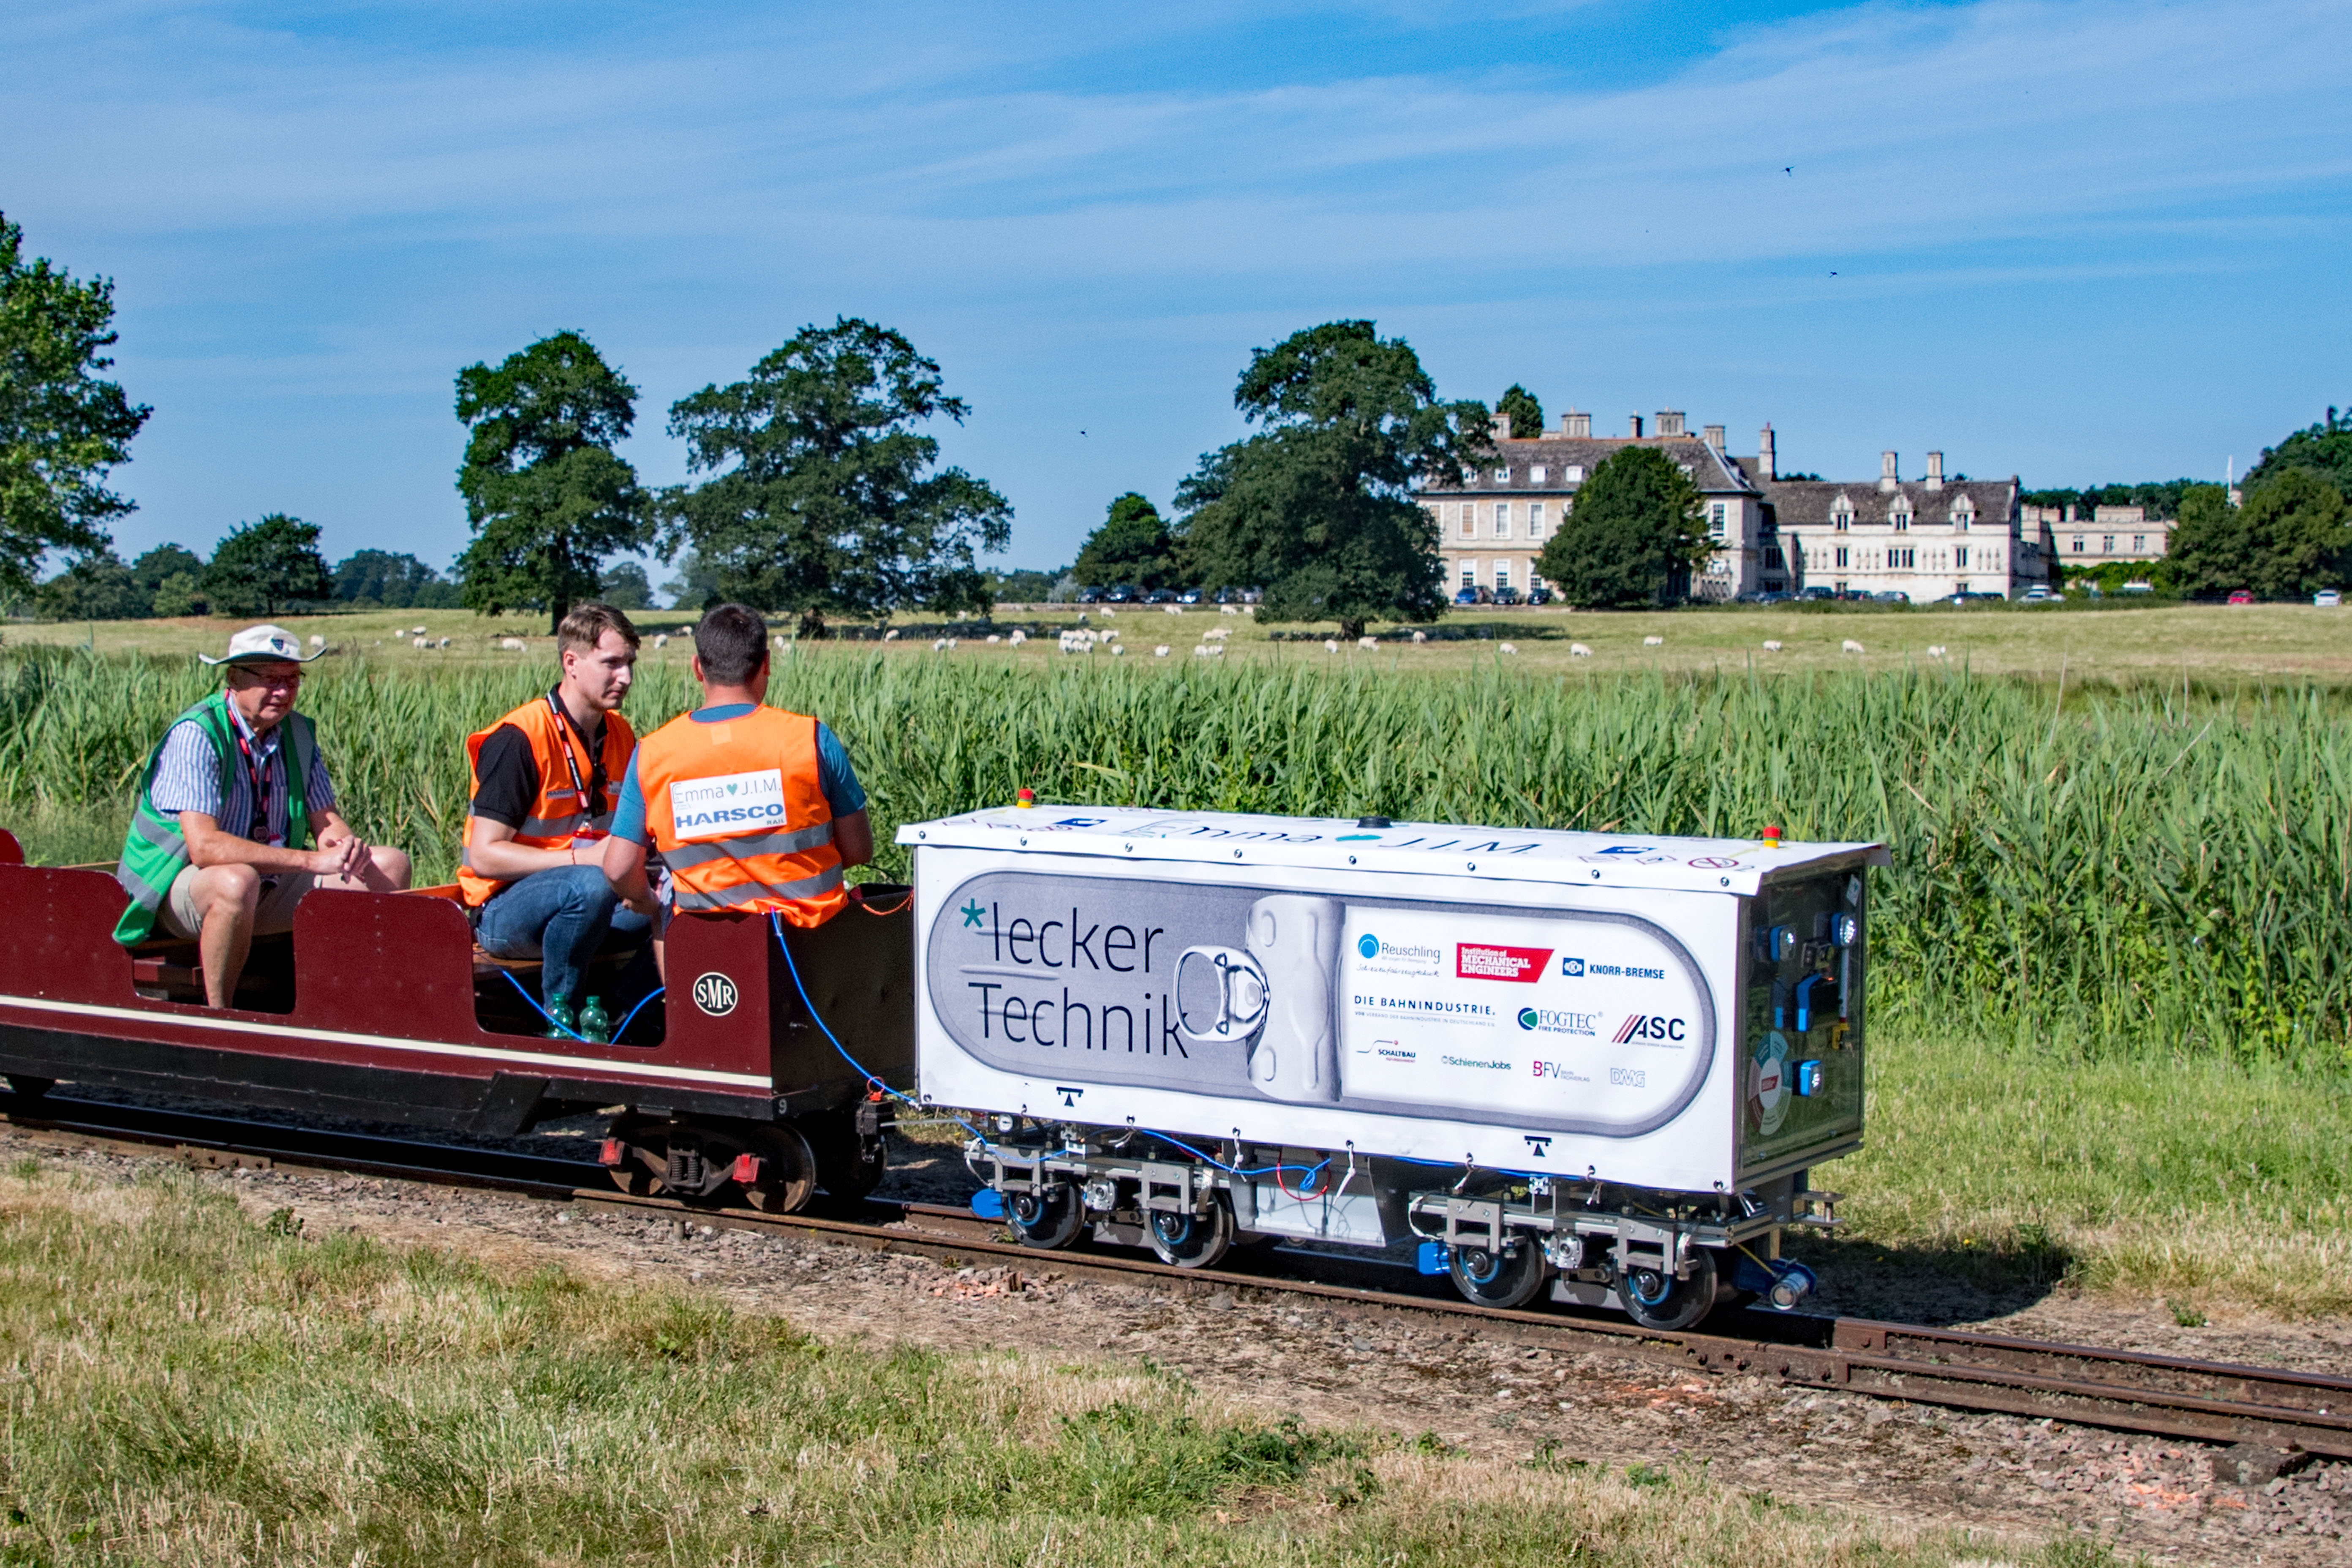
\includegraphics[width= \paperwidth]{EmmaCastle.jpg}}
%
%\section{IMechE Railway Challenge}
%\frame{\vspace{1cm}
%
%\begin{center}
% \color{white} \usebeamerfont{title}{IMechE Railway Challenge}
%\end{center}
%}
%}
%
%
%\frame{\frametitle{Was ist die IMechE Railway Challenge?}
%\framesubtitle{Die IMechE nutzt viele Kan\"ale, um junge Menschen f\"ur die Eisenbahn zu begeistern, die Railway Challenge ist einer davon.}
%\begin{columns}[t] 
%     \begin{column}[T]{7cm} 
%     	\begin{itemize}
%     		\item Wettbewerb auf Parkbahnanlage:
%		\begin{itemize}
%		\item Relevante Disziplinen, z.B. 
%		\begin{itemize}
%		\item L\"armreduzierung
%		\item Energier\"uckgewinnung
%		\item Innovation
%		\item Business Case
%		\end{itemize}
%		\end{itemize}
%		\item Raum f\"ur Innovation:
%		\begin{itemize}
%		\item H$_{2}$-Brennstoffzelle
%		\item IoT-Connection
%		\item Autonomes Fahren (geplant f\"ur 2019)
%		\end{itemize}
%		\item FH Aachen ist erster ``Overseas Entry''
%     	\end{itemize}
%     \end{column}
%     	\begin{column}[T]{7cm} 
%         	\begin{center}
%	\vspace{-1cm}
%            		\includegraphics[width=0.7\textwidth]{EmmaSeite}
%        		\end{center}
%     \end{column}
% \end{columns}
%}
%
%\frame{\frametitle{Welchen Vorteil haben die Studierenden?}
%\framesubtitle{Das Erlernte kann sofort in die Praxis eingebracht werden, es kann diskutiert, geschraubt, get\"uftelt und getestet werden. Durch die Abbildung des gesamten Lebenszyklus' ist f\"ur jeden etwas dabei!}
%\begin{columns}[t] 
%     \begin{column}[T]{7cm} 
%     	\begin{itemize}
%     		\item Praxiserfahrung
%		\item Vernetzung
%		\item Roter Faden durch Lehrveranstaltungen und Praktika
%		\item Internationalit\"at
%		\item Vertiefung ohne B\"uffeln
%		\item Sich ausprobieren k\"onnen
%		\item Erfolge genie{\ss}en
%		\item Aus Misserfolgen lernen
%		\item Spa{\ss}!
%     	\end{itemize}
%     \end{column}
%     	\begin{column}[T]{7cm} 
%         	\begin{center}
%		\vspace{-.5cm}
%            		\href{https://www.youtube.com/watch?v=_z9fII6lbig}{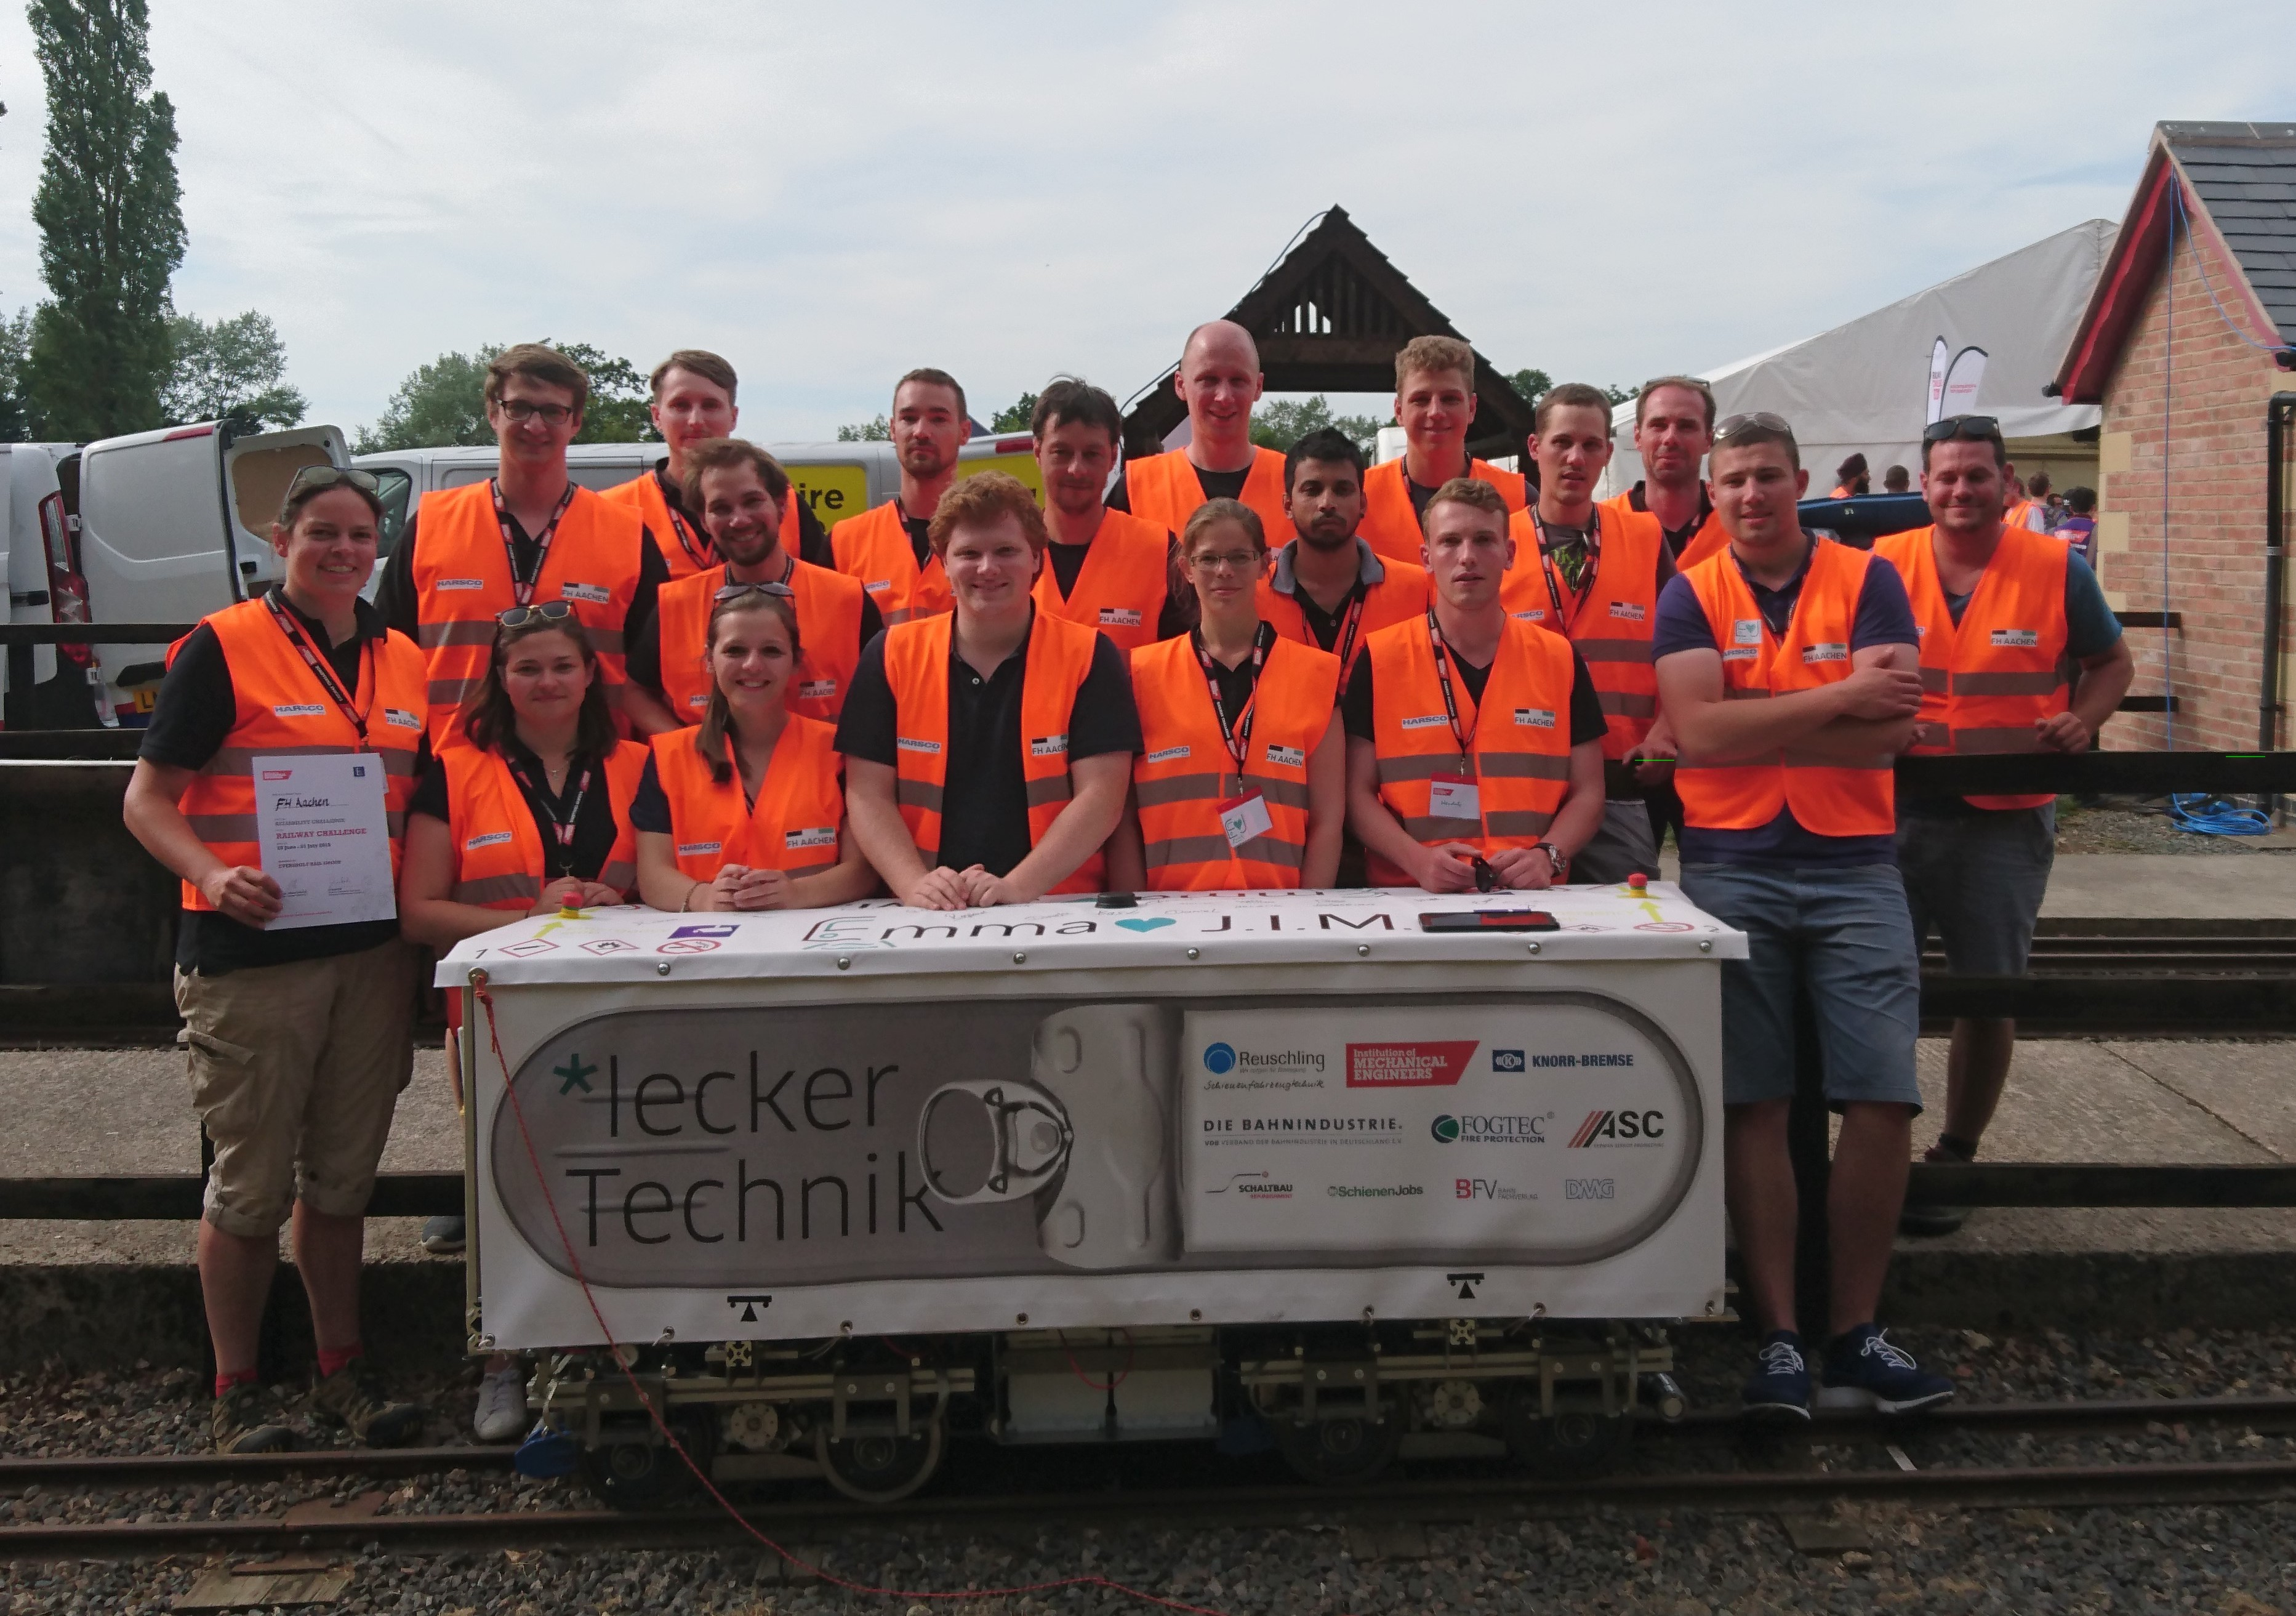
\includegraphics[width=0.9\textwidth]{Winners2018}}\\
%			Team FH$_{2}$Rail\\
%			IMechE Railway Challenge 2018\\ \vspace{.5cm}
%			4. Platz von 12 Teilnehmern
%        		\end{center}
%     \end{column}
% \end{columns}
%}
%
%\frame{\frametitle{Sponsoring f\"ur Emma und das Team?}
%\framesubtitle{}
%\begin{columns}[t] 
%     \begin{column}[T]{7cm} 
%     	\begin{itemize}
%     		\item Nationale und internationale Sichtbarkeit (Youtube, Facebook, Innotrans, ...)
%%		\begin{itemize}
%%		\item Marke
%%		\item Technologie
%%		\end{itemize}
%		\item Engagement im Bereich Nachwuchsgewinnung
%		\item Direkten Kontakt zu Studierenden
%		\item Studierende in Ber\"uhrung mit eigenen Technologien bringen
%		\item Sponsoring Pakete:
%		\begin{itemize}
%		\item Namenssponsor (5000 \euro) (verkauft)
%		\item Logo auf Lok (500/1000 \euro)
%		\item Warnwesten-Sponsor (2000 \euro)
%		\item Dinner-Sponsor (800 \euro) (verkauft)
%		\end{itemize}
%		\item F\"ur alle Pakete: Sponsoren-Event mit Studierenden
%     	\end{itemize}
%     \end{column}
%     	\begin{column}[T]{7cm} 
%         	\begin{center}
%            		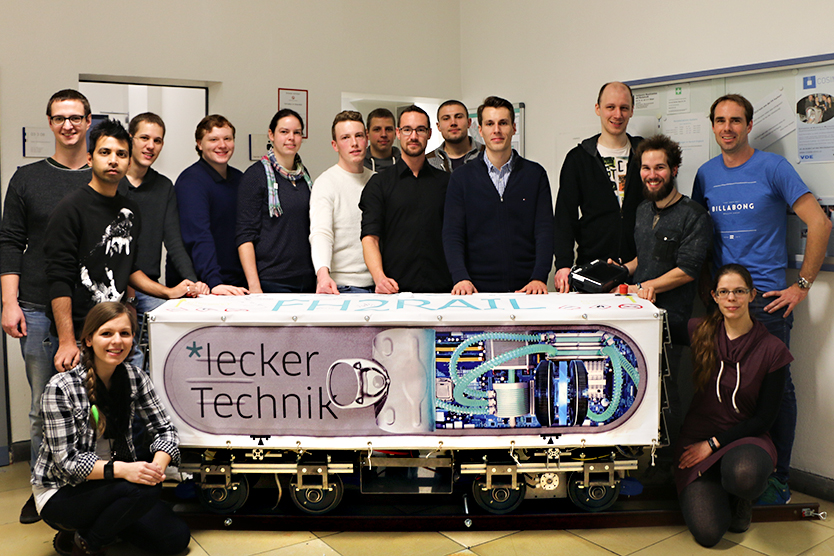
\includegraphics[width=0.9\textwidth]{Team2018}\source{}
%		Team Emma {\Large \color{mint!90!black}$\varheartsuit$} J.I.M. \\
%		IMechE Railway Challenge 2018\\ \vspace{.5cm}
%		www.emmalovesjim.com
%        		\end{center}
%     \end{column}
% \end{columns}
%}
%
%\frame{\frametitle{Was Emma braucht, um erfolgreich zu sein...}
%\framesubtitle{}
%\begin{columns}[t] 
%     \begin{column}[T]{6cm} 
%     	\begin{itemize}
%     		\item<1-> Motivierte Studis
%		\item<2-> Viel Liebe
%		\item<3-> Leere Bierkisten
%		\item<4-> Viel mehr Probefahrten
%		\only<5->{\item Hardware, insbesondere:
%		\begin{itemize}
%		\item Camera und Laserscanner
%		\item Kompakte Batterien
%		\item Federspeicherbremsen
%		\item Kompressor
%		\item 4G/WiFi Connection
%		\item Sandungssystem
%		\end{itemize}
%		}
%     	\end{itemize}
%	%\only<6>{2019 mit Ihnen als Sponsor?}
%     \end{column}
%     	\begin{column}[T]{8cm} 
%         	\begin{center}
%            		\only<1>{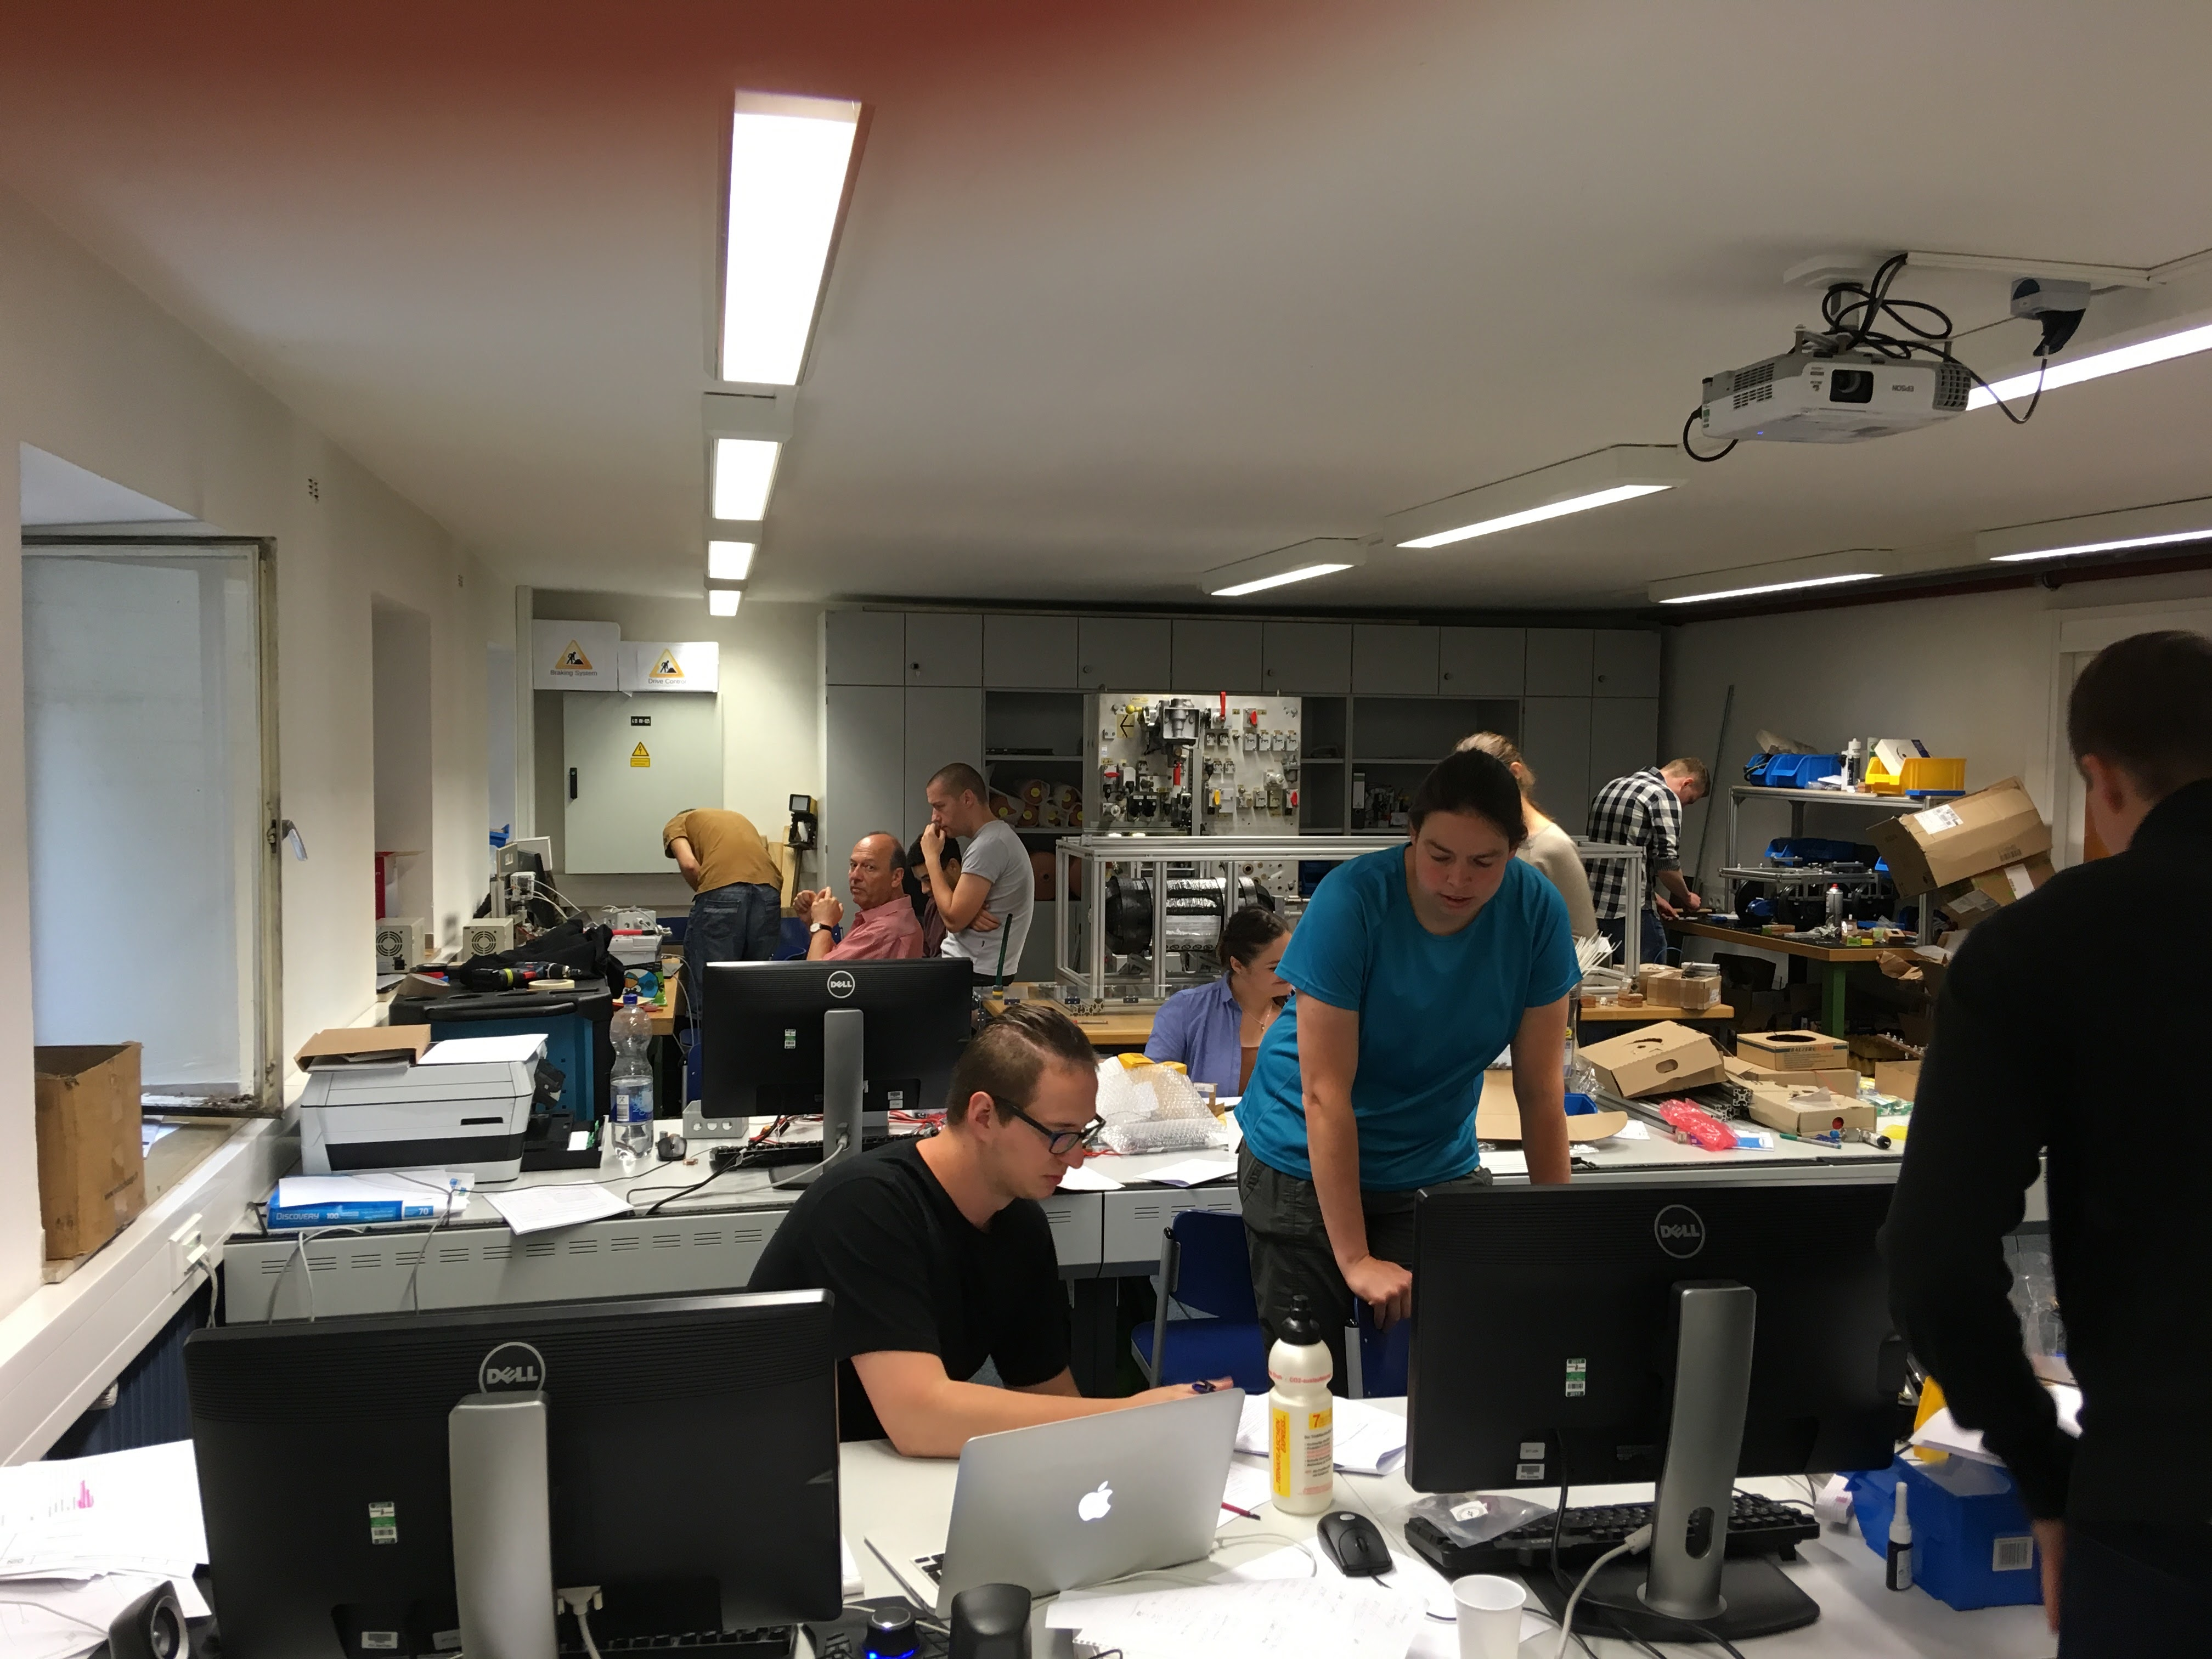
\includegraphics[width=1\textwidth]{IMG_0845}}
%			\only<2>{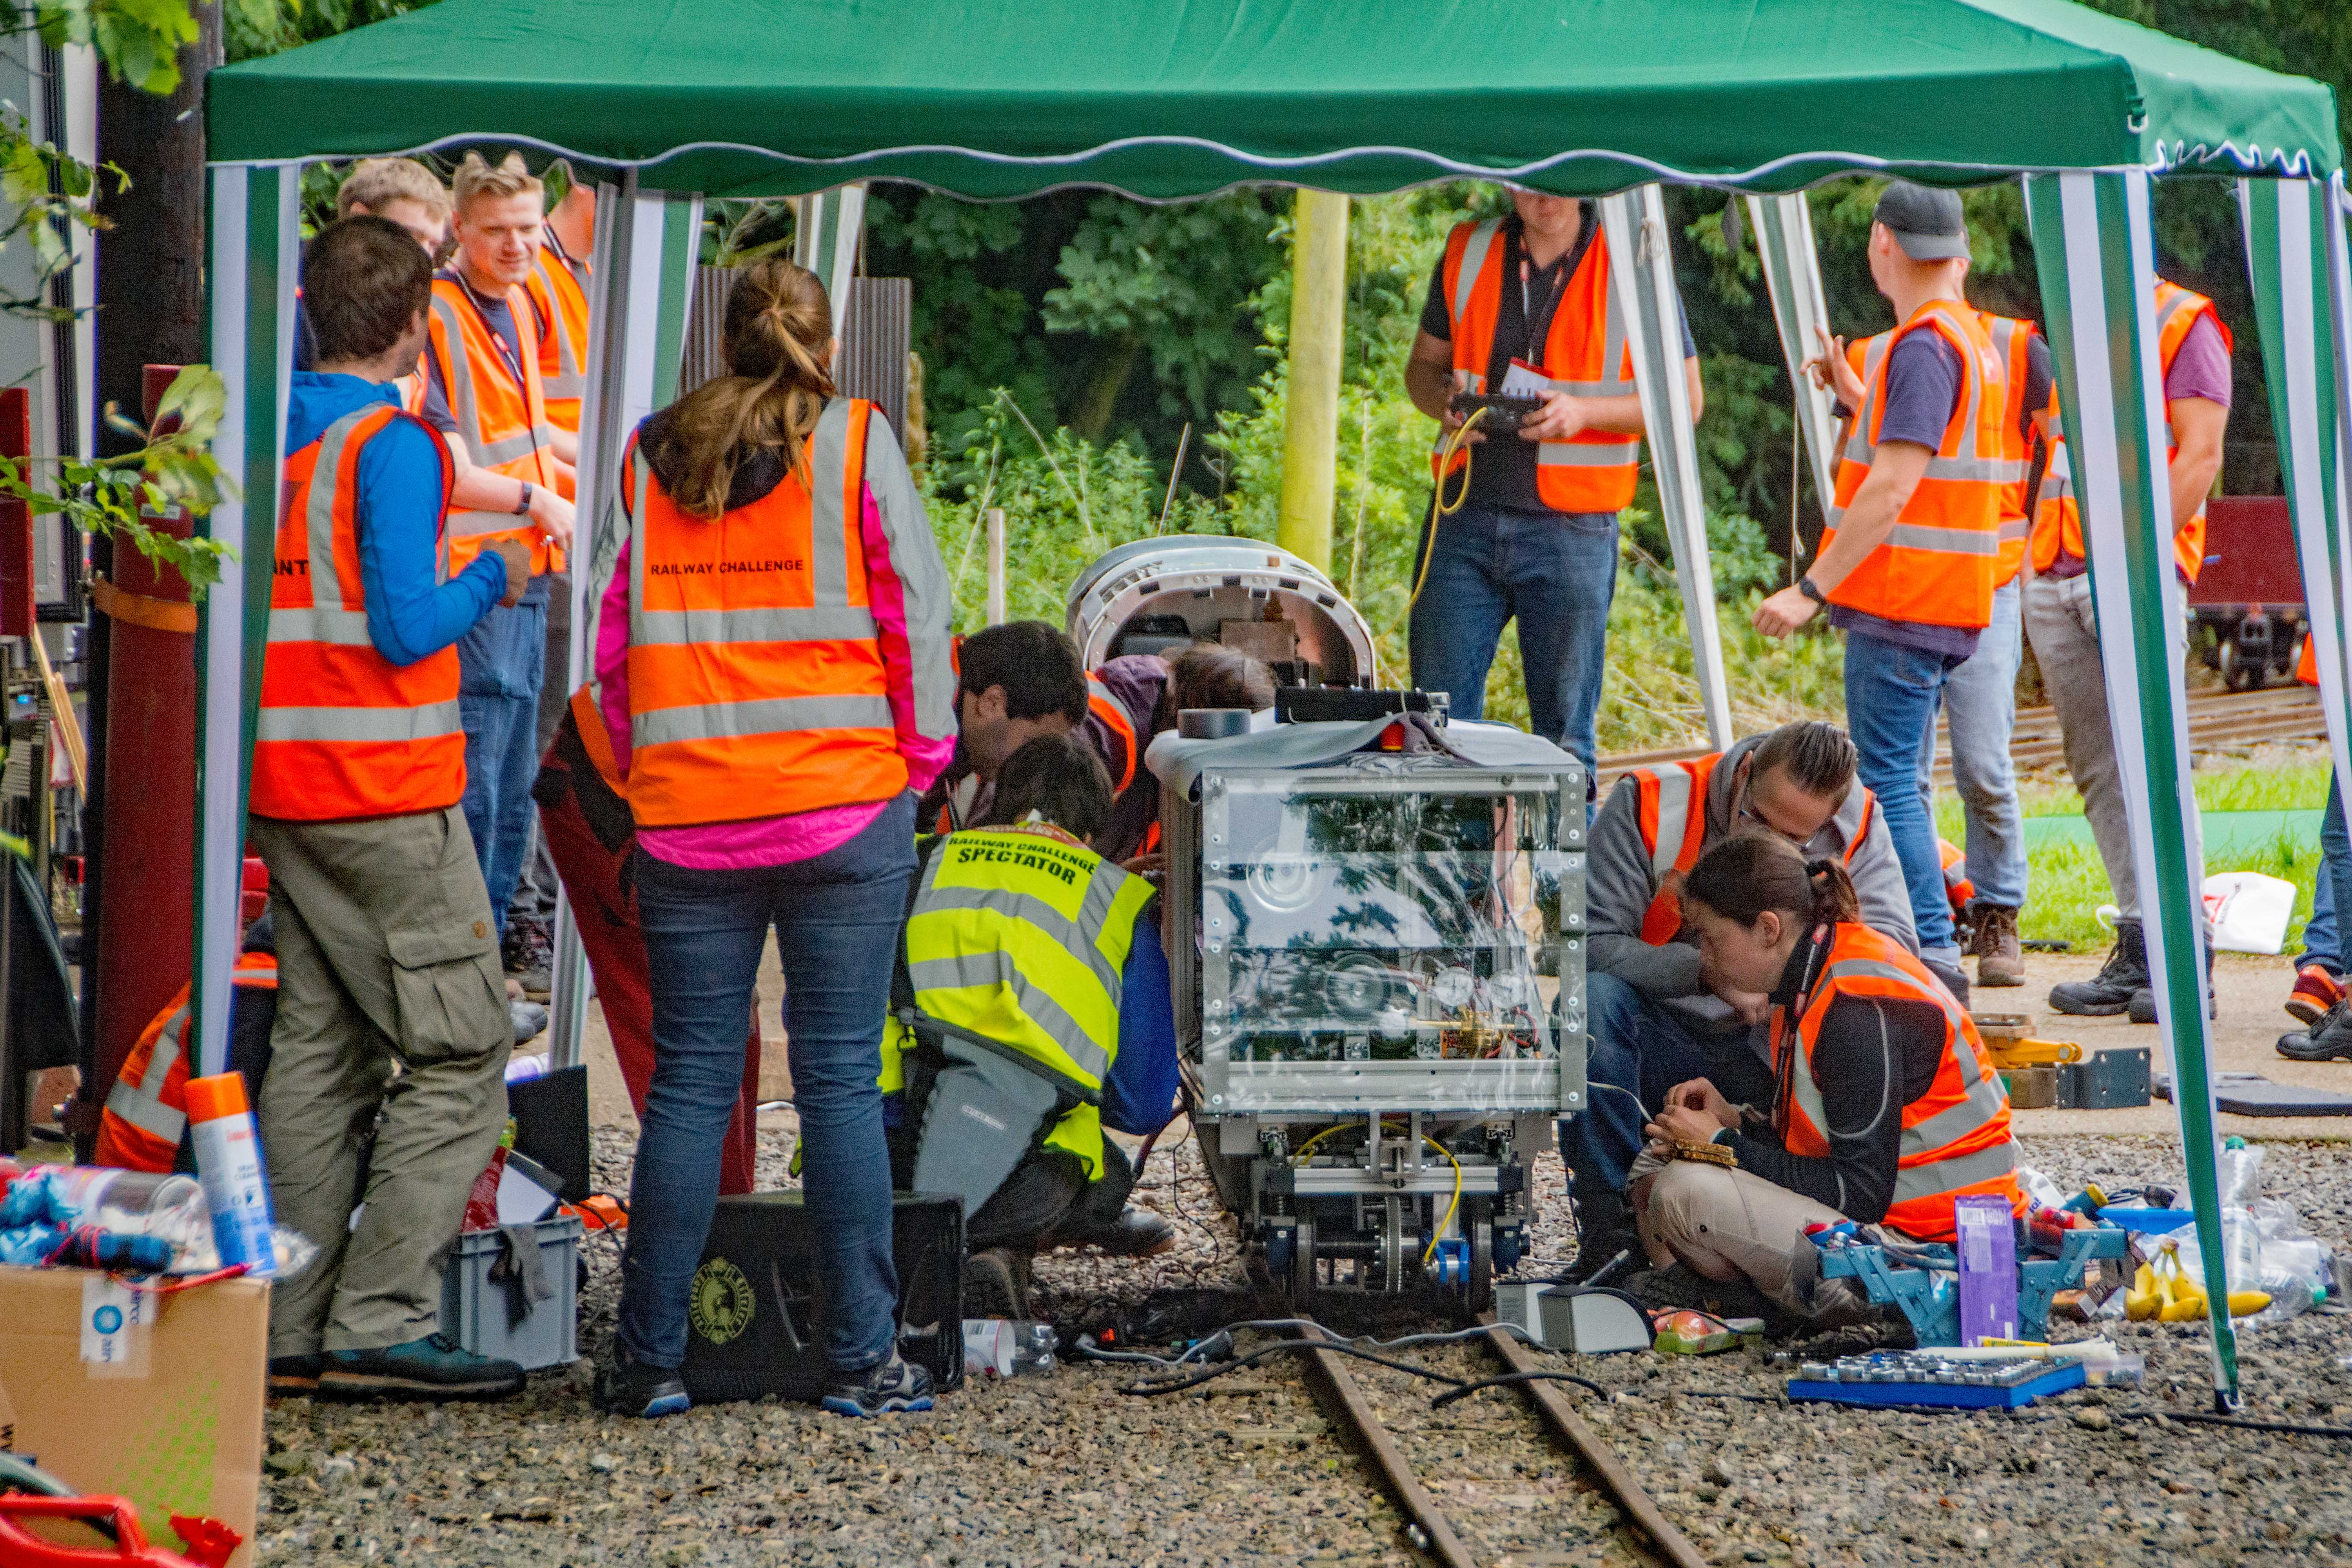
\includegraphics[width=1\textwidth]{DSC_1375}}
%			\only<3>{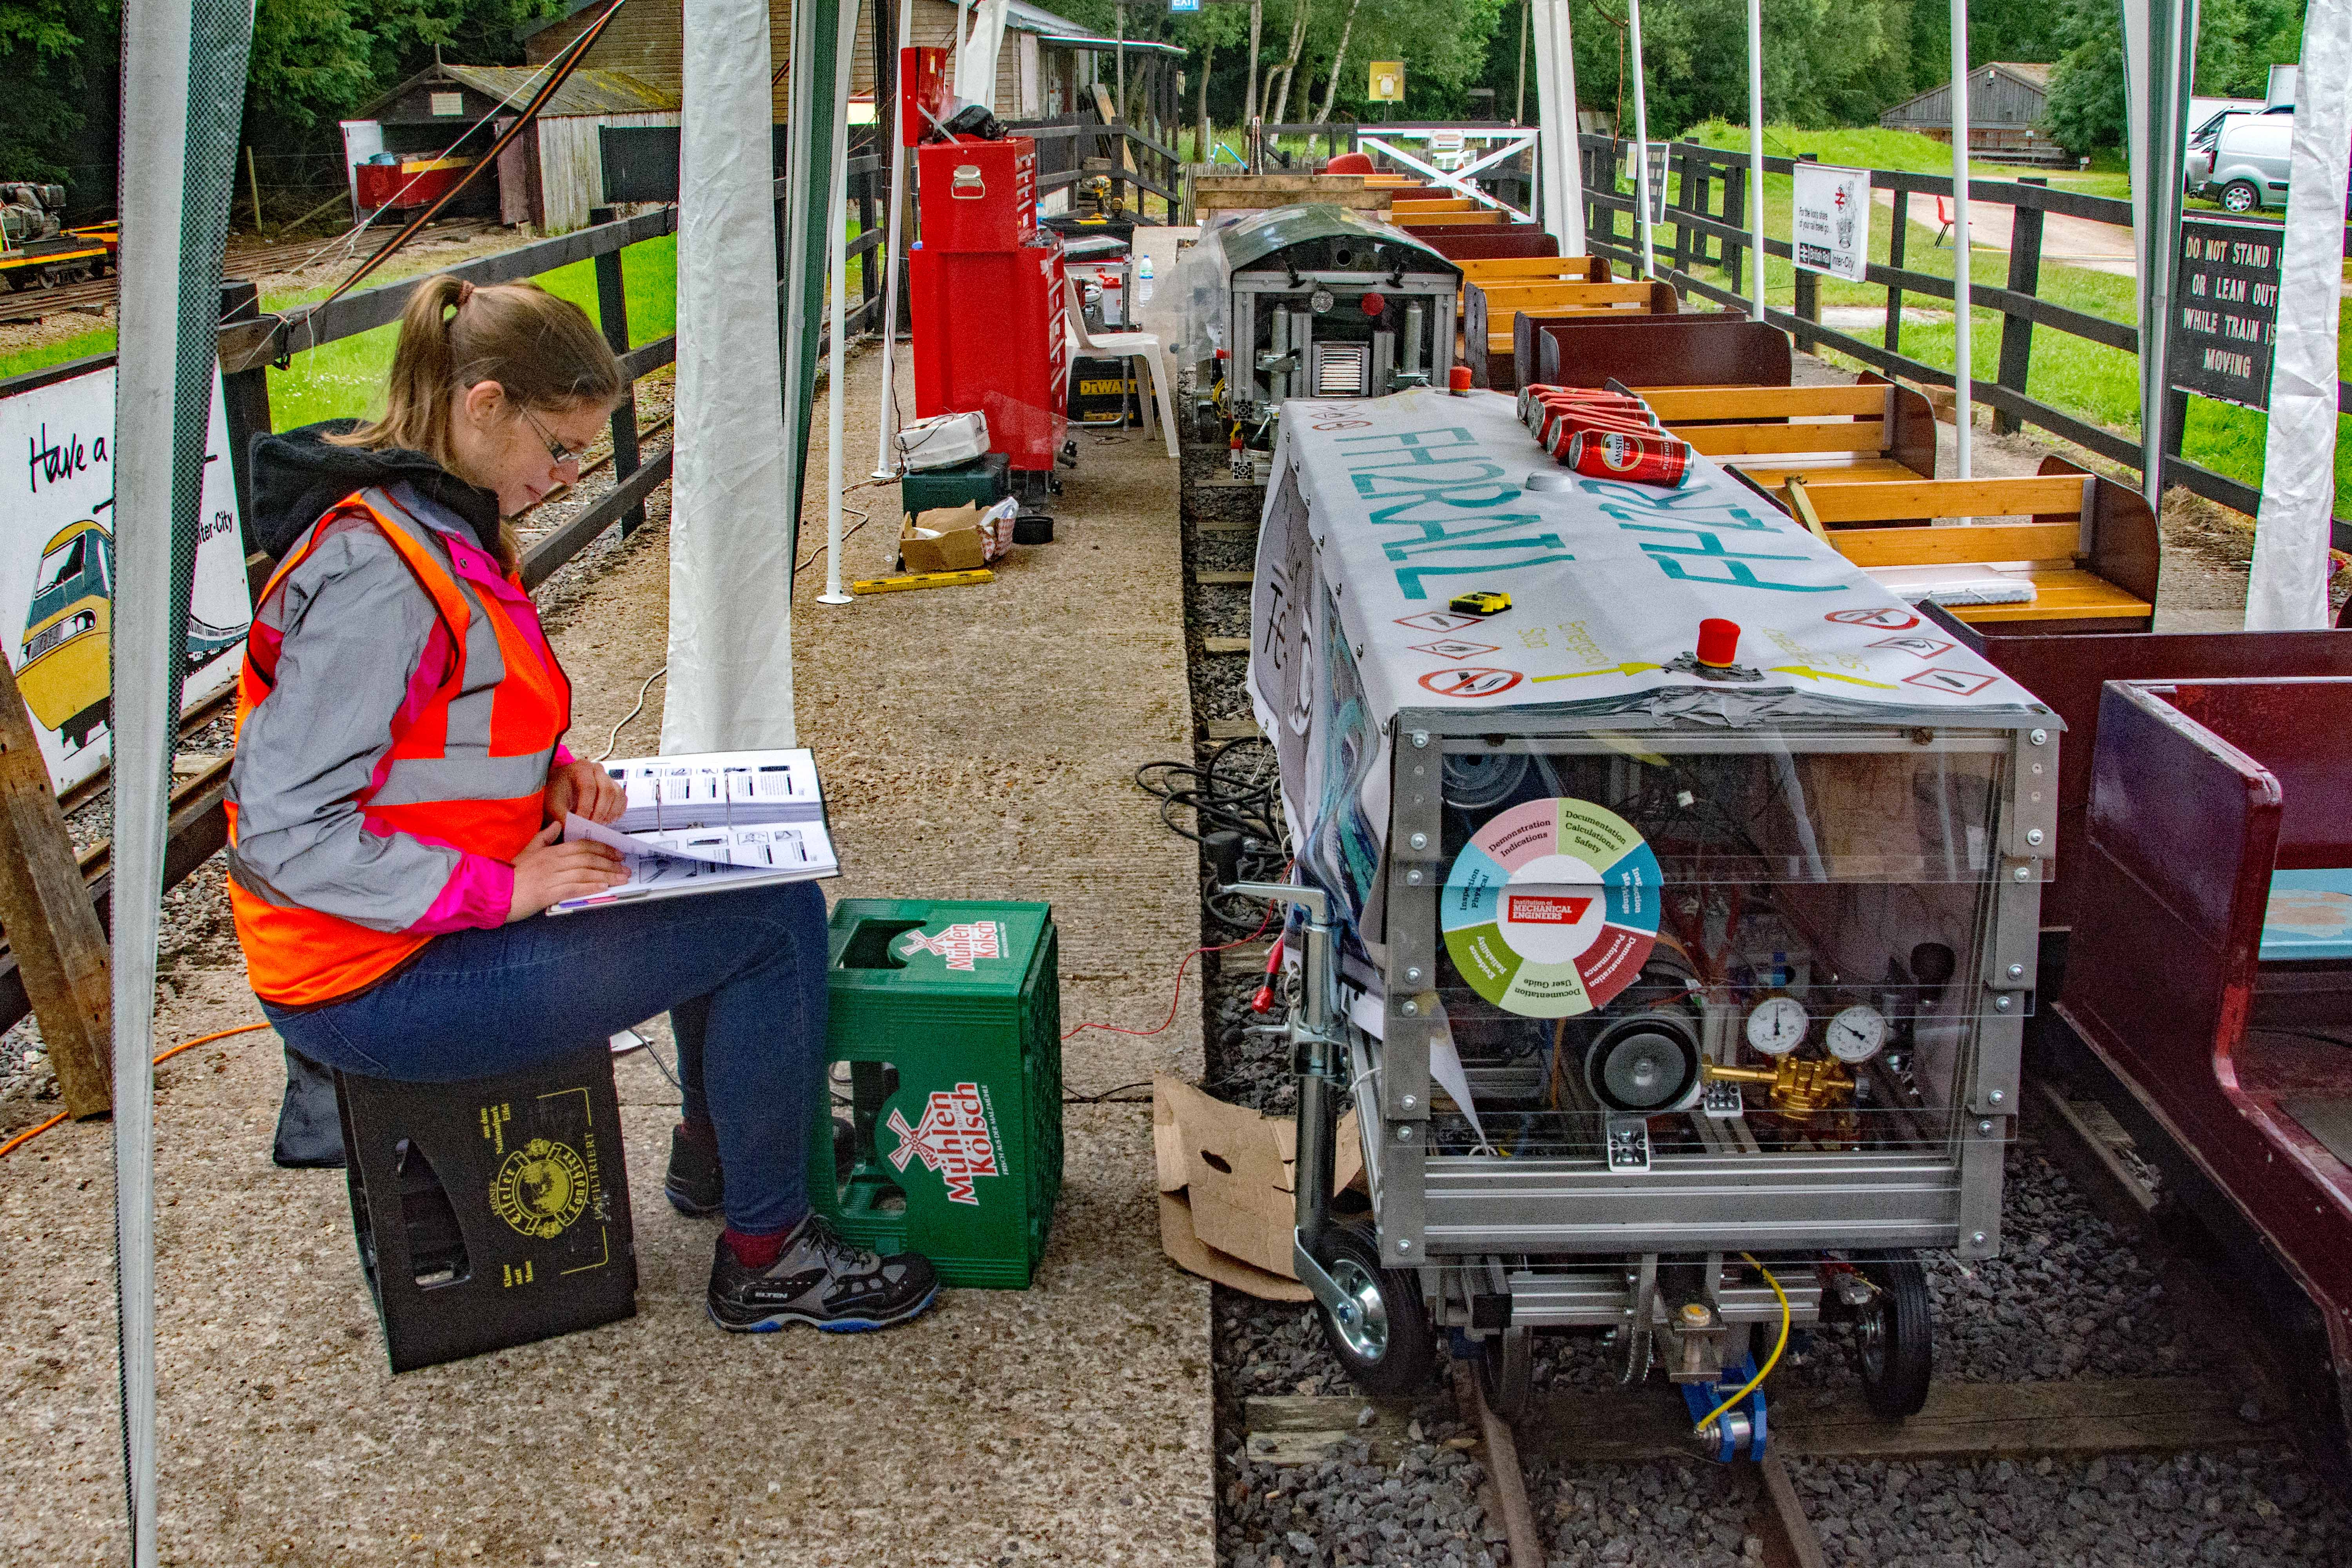
\includegraphics[width=1\textwidth]{DSC_1777}}
%			\only<4>{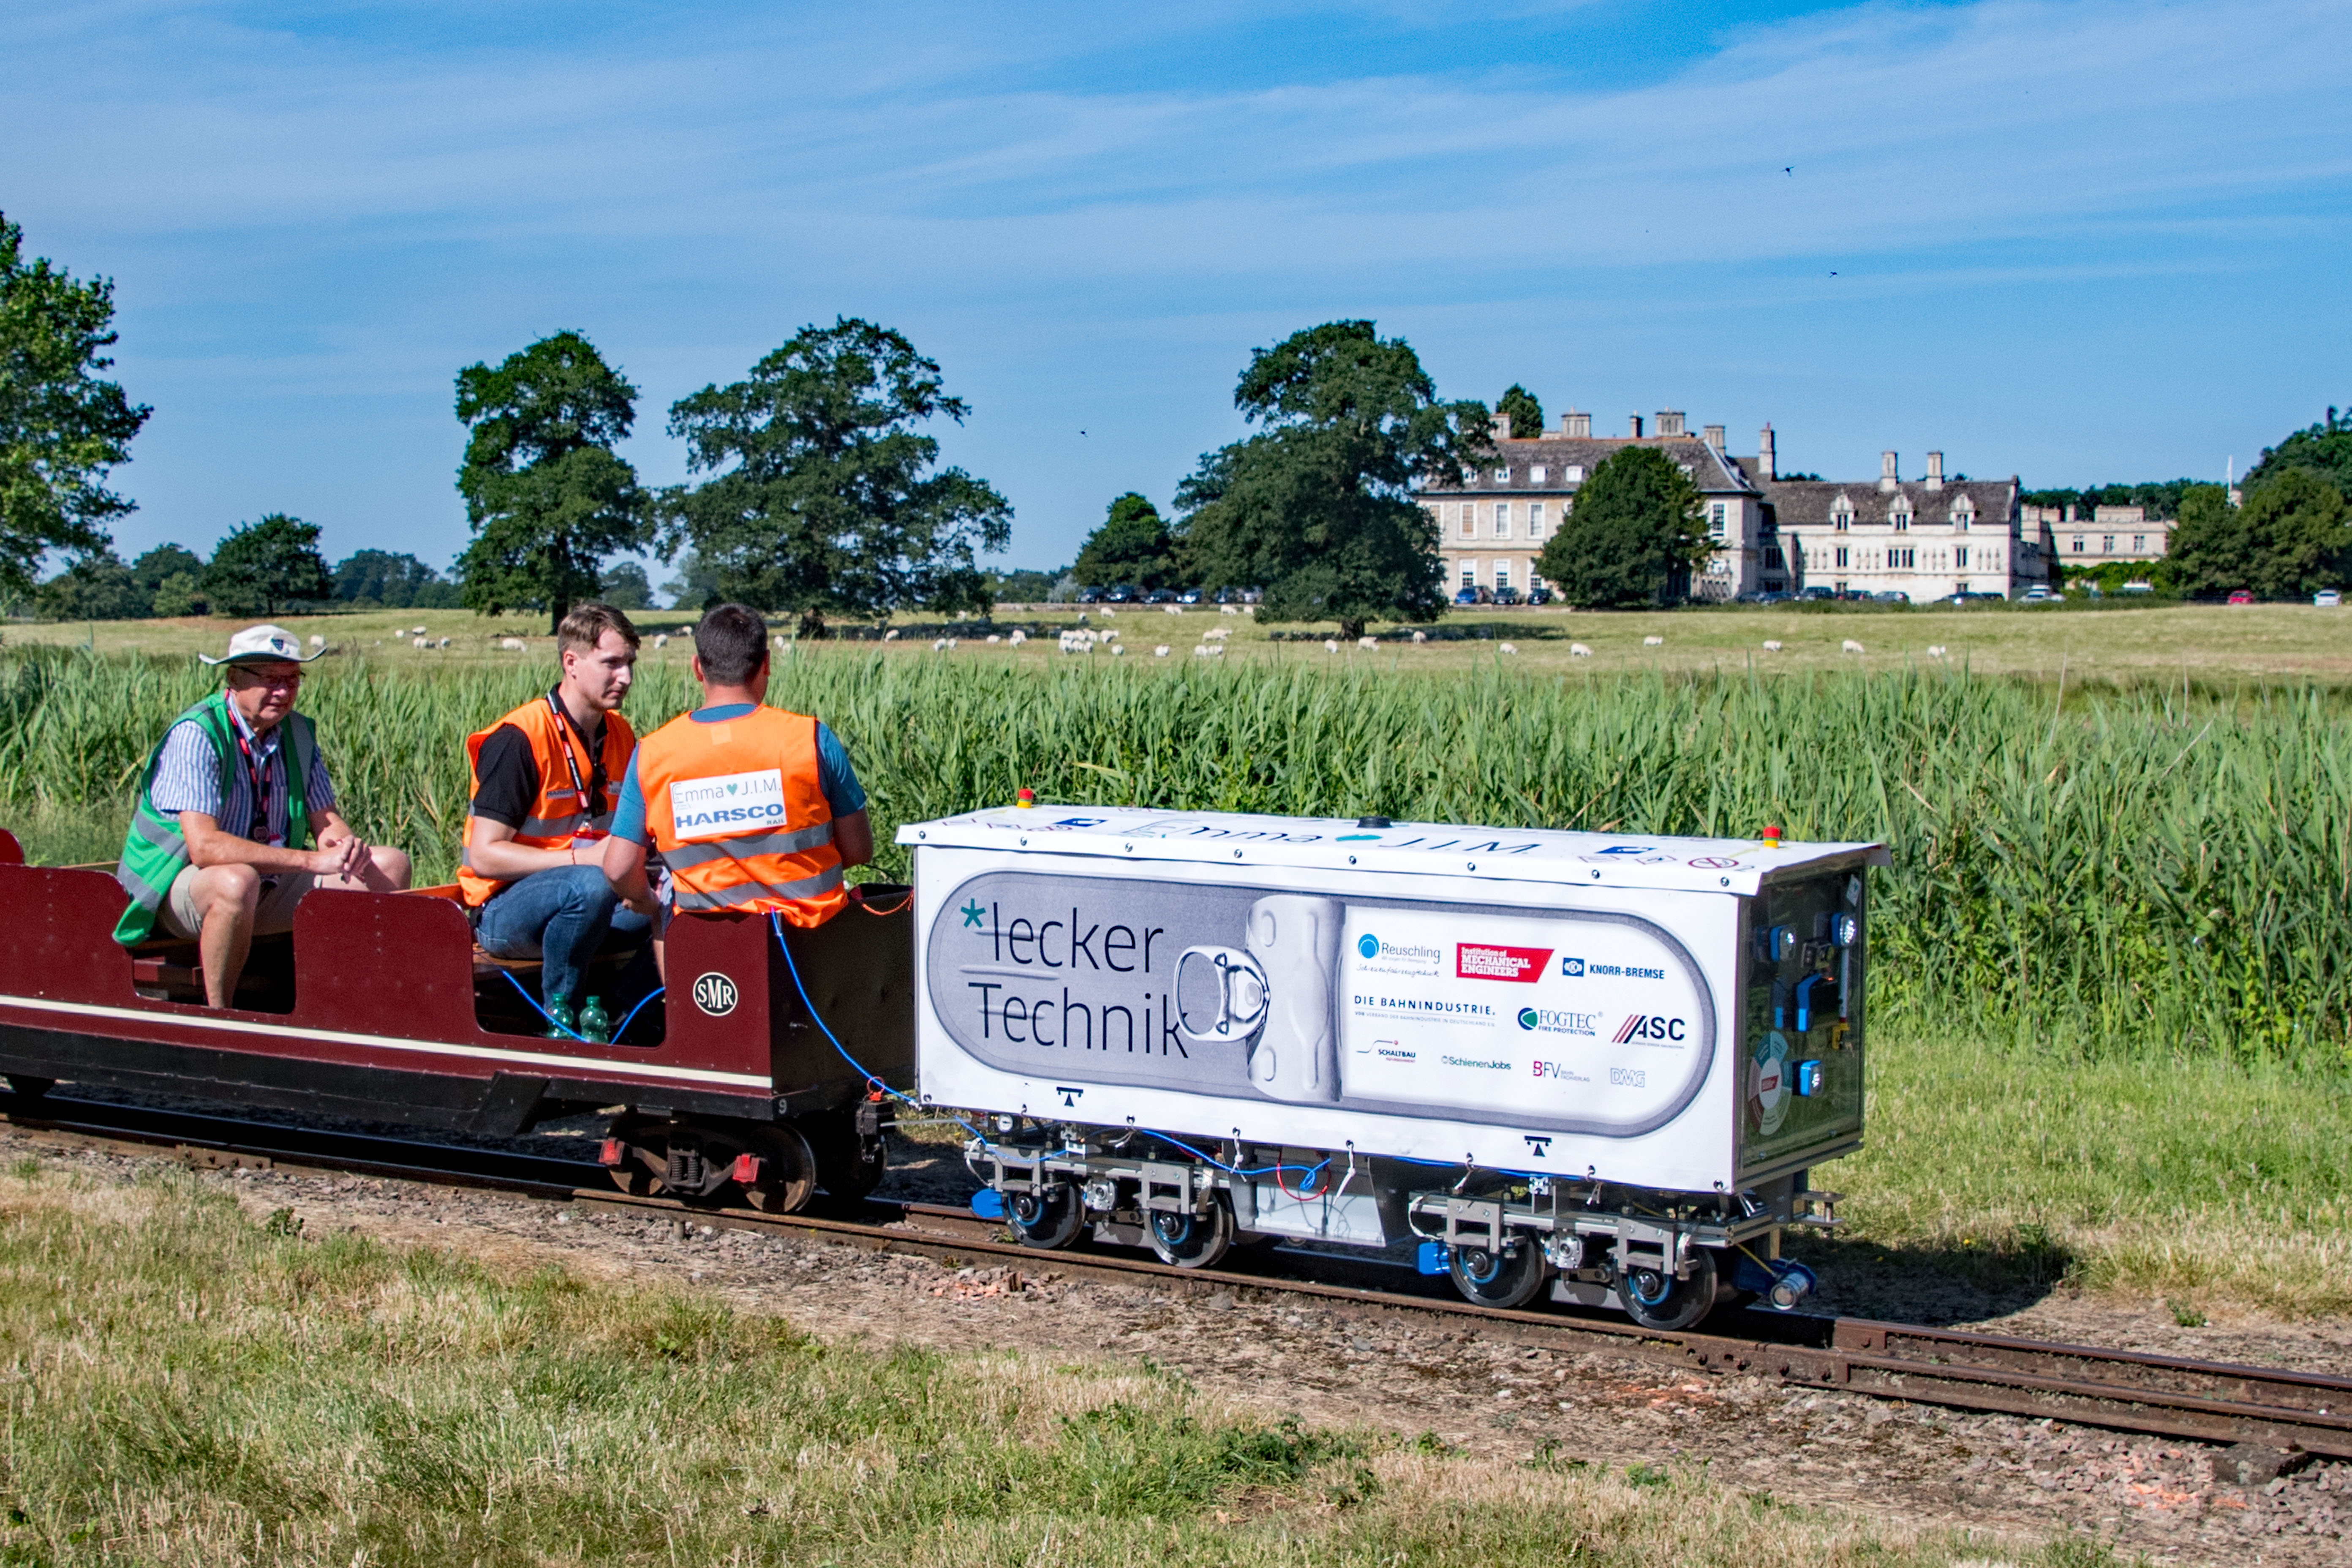
\includegraphics[width=1\textwidth]{EmmaCastle}}
%			\only<5->{\vspace{-.5cm}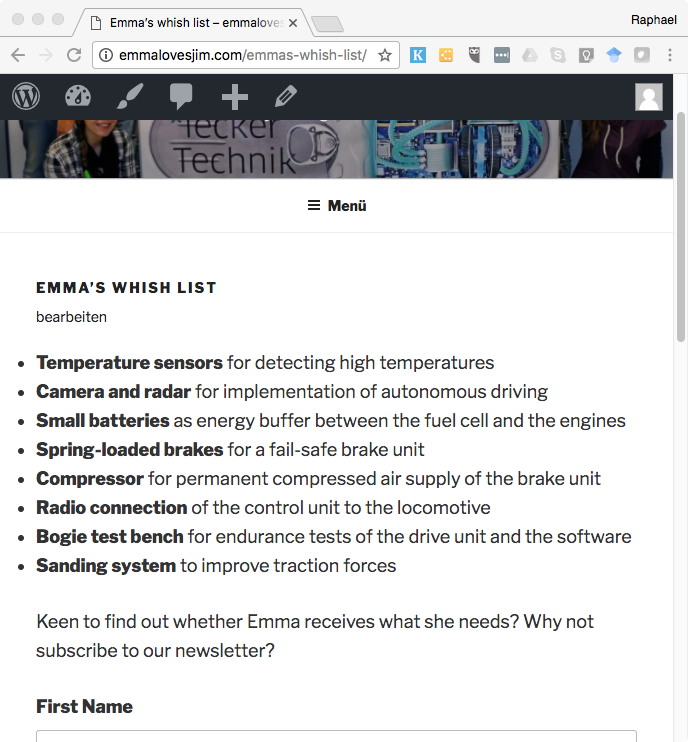
\includegraphics[width=.9\textwidth]{Whishlist}}
%        		\end{center}
%     \end{column}
% \end{columns}
%}
%
%{
%\usebackgroundtemplate{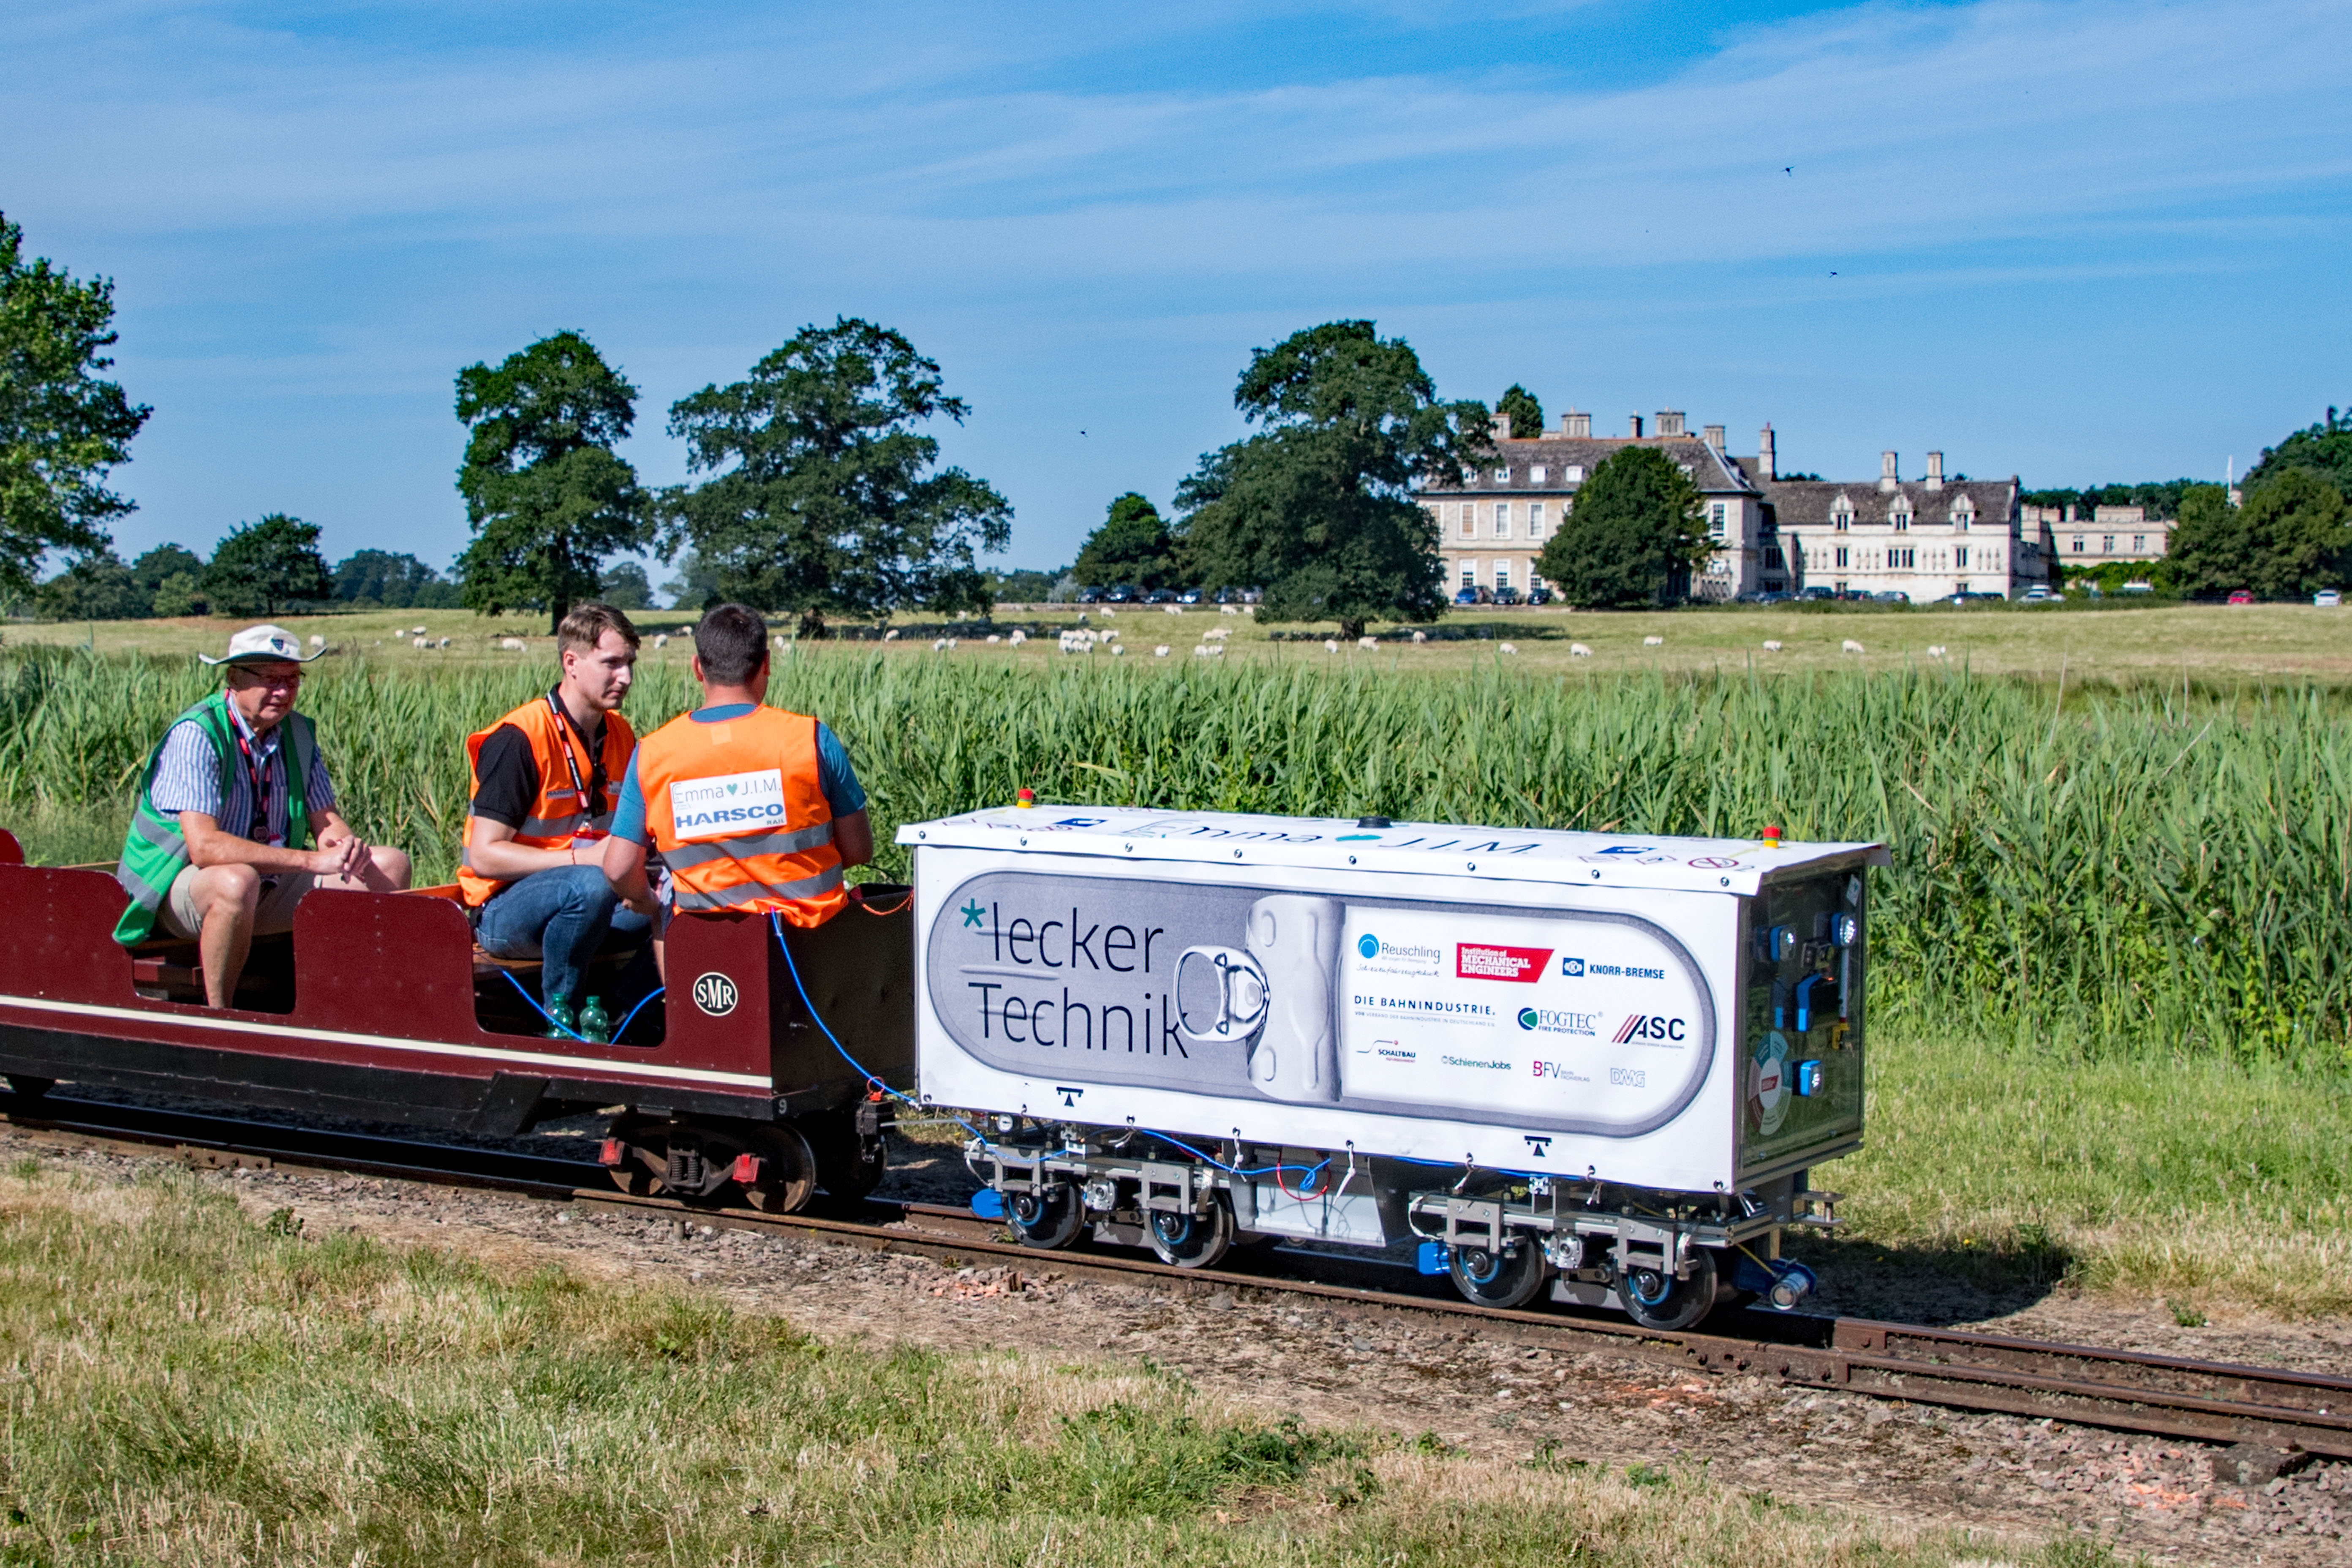
\includegraphics[width= \paperwidth]{EmmaCastle.jpg}}
%
%\frame{\frametitle{\color{white}Was k\"onnen Emma und das Team der Bahnindustrie geben?}
%\framesubtitle{}
%\begin{itemize} \color{white}
%\item Neues Bild von Studium und Beruf im Bereich Bahn
%\item Jugendliche Darstellung
%\item ``Du bist hier willkommen!''
%\item ``Du kannst etwas ausprobieren und etwas bewegen!''
%\item ``Coole Technik hier - und sinnvoll ist es auch!''
%\end{itemize}
%\vspace{-0.5cm}
%\only<2>{\begin{center}
%\Huge \textbf{%\color{mint!75!black}
%Dabei hilft Ihr Engagement!}
%\end{center}}
%}
%}
%
{
\usebackgroundtemplate{\transparent{0.4}\includegraphics[width= 1.2\paperwidth]{Lecker}}

\frame{\frametitle{Let's put awesome back into railways!}
\begin{center}
			\vspace{5.5cm}
            		%\includegraphics[width=.8\textwidth]{Lecker}
        		\end{center}
\begin{columns}[t] 
\begin{column}[T]{1cm} 
     	\end{column}
     \begin{column}[T]{7cm} 
     
     	%\includegraphics[width = .25 \textwidth]{SlidesVDB}
     \end{column}
     	\begin{column}[T]{7cm} 
		{\color{white}
		\textbf{Prof. Dr. Raphael Pfaff\\
		%Rail vehicle engineering\\
		pfaff@fh-aachen.de\\
		www.raphaelpfaff.net}}
     \end{column}
 \end{columns}
}
}
\end{document}
